\section{Algoritmo de Bellman-Ford}

\begin{frame}[fragile]{Caminhos mínimos}

    \begin{itemize}
        \item Seja $G(V, E)$ um grafo e $u, v\in V$. Um caminho de $u$ a $v$ é uma sequência de
            $M$ arestas $p = \lbrace (a_0, a_1), (a_1, a_2), \ldots, (a_{M-1}, a_M)\rbrace$ tal que
            $a_0 = u, a_M = v$ e, para cada par $a, b$ de arestas consecutivas de $p$, o 
            segundo vértice de $a$ é igual ao primero vértice de $b$

        \item O conjunto $C$ de todos os caminhos de $u$ a $v$ é dado por
        \[
            C(u, v) = \lbrace p\subset E\ |\ p\ \mbox{é caminho de}\ u\ \mbox{a}\ v\rbrace
        \]

        \item Se $C(u, v)\neq \emptyset$, o caminho de custo mínimo, ou simplesmente caminho 
        mínimo, de 
        $u$ a $v$ é um caminho, é o elemento de $m\in C$ tal que a soma dos pesos da arestas 
        da sequência $m$ é a menor possível

        \item Se o grafo não é ponderado, o caminho mínimo entre $u$ e $v$ pode ser obtido
            através de uma BFS
    \end{itemize}

\end{frame}

\begin{frame}[fragile]{Algoritmo de Bellman-Ford}

    \begin{itemize}
        \item O algoritmo de Bellman-Ford computa o caminho mínimo de todos os vértices de
            um grafo a um nó $s$ dado

        \item É um algoritmo versátil, que pode processar grafos cujas arestas podem ter pesos
            negativos

        \item O único tipo de grafo que ele não processa são grafos com ciclos negativos,
            mas é capaz de detectar tais grafos

        \item Inicialmente, ele inicializa a distance de $s$ a $s$ como zero e igual a
            infinito para todos os demais nós

        \item A cada iteração, ele visita todas as arestas na tentativa de encurtar um
            caminho já existente, até que não seja mais possível esta redução

        \item A complexidade é $O(VE)$, pois o número de arestas máximo em um caminho mínimo é
            igual a $V - 1$
    \end{itemize}

\end{frame}

\begin{frame}[fragile]{Visualização do algoritmo de Bellman-Ford}

    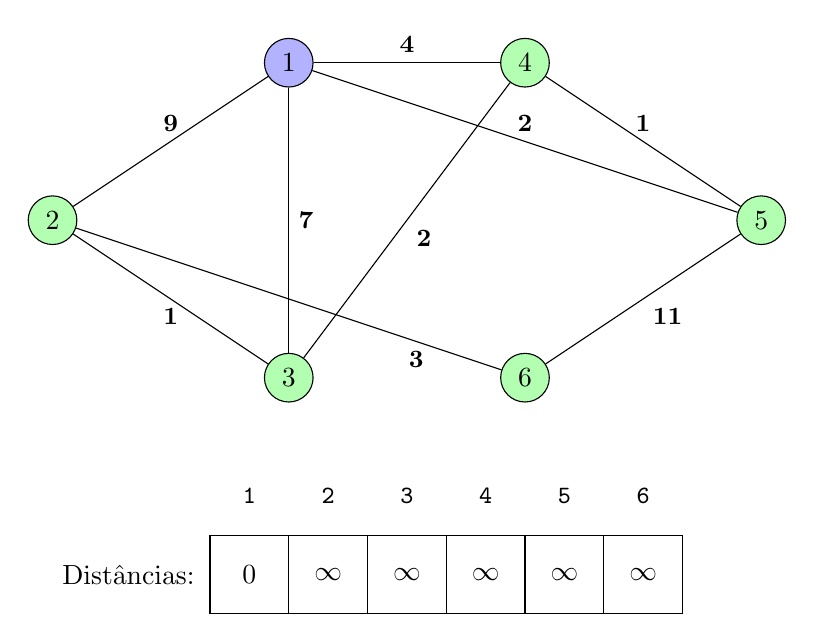
\begin{tikzpicture}
        \node[anchor=west] at (0, 0.5) { Distâncias: };

        \node[circle, draw, fill=blue!30] (a) at (3, 7) {1};
        \node[circle, draw, fill=green!30] (b) at (0, 5) {2};
        \node[circle, draw, fill=green!30] (c) at (3, 3) {3};
        \node[circle, draw, fill=green!30] (d) at (6, 7) {4};
        \node[circle, draw, fill=green!30] (e) at (9, 5) {5};
        \node[circle, draw, fill=green!30] (f) at (6, 3) {6};

        \draw (2, 0) grid (8, 1);

        \node at (2.5, 0.5) { $0$ };
        \node at (3.5, 0.5) { $\infty$ };
        \node at (4.5, 0.5) { $\infty$ };
        \node at (5.5, 0.5) { $\infty$ };
        \node at (6.5, 0.5) { $\infty$ };
        \node at (7.5, 0.5) { $\infty$ };

        \node at (2.5, 1.5) { \small \texttt{1} };
        \node at (3.5, 1.5) { \small \texttt{2} };
        \node at (4.5, 1.5) { \small \texttt{3} };
        \node at (5.5, 1.5) { \small \texttt{4} };
        \node at (6.5, 1.5) { \small \texttt{5} };
        \node at (7.5, 1.5) { \small \texttt{6} };

        \draw (a) to node[midway,anchor=south] { \small \bfseries 9 } (b);
        \draw (a) to node[midway,anchor=west] { \small \bfseries 7 } (c);
        \draw (a) to node[midway,anchor=south] { \small \bfseries 4 } (d);
        \draw (a) to node[midway,anchor=south] { \small \bfseries 2 } (e);
        \draw (b) to node[midway,anchor=north] { \small \bfseries 1 } (c);
        \draw (b) to node[pos=0.8,anchor=north] { \small \bfseries 3 } (f);
        \draw (c) to node[midway,anchor=north west] { \small \bfseries 2 } (d);
        \draw (d) to node[midway,anchor=south] { \small \bfseries 1 } (e);
        \draw (e) to node[midway,anchor=north west] { \small \bfseries 11 } (f);

    \end{tikzpicture}

\end{frame}

\begin{frame}[fragile]{Visualização do algoritmo de Bellman-Ford}

    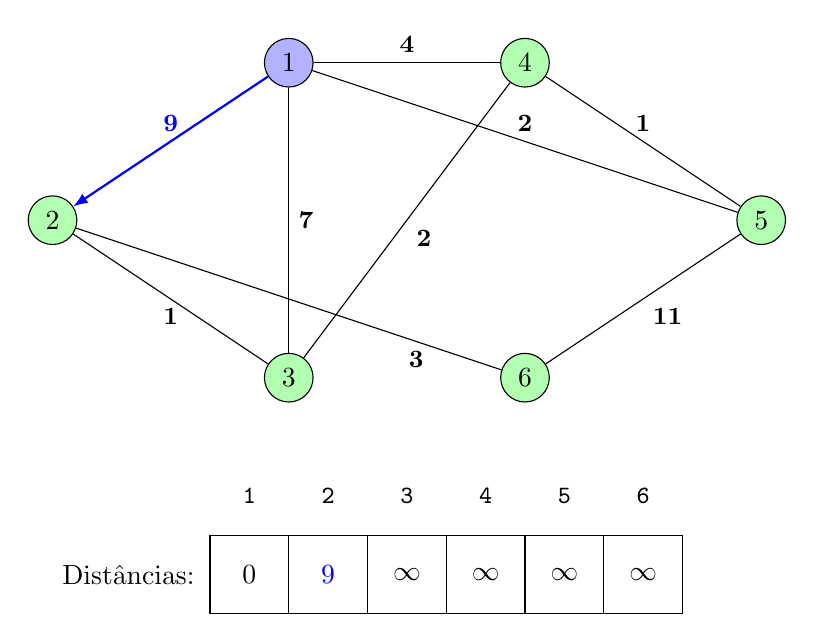
\begin{tikzpicture}
        \node[anchor=west] at (0, 0.5) { Distâncias: };

        \node[circle, draw, fill=blue!30] (a) at (3, 7) {1};
        \node[circle, draw, fill=green!30] (b) at (0, 5) {2};
        \node[circle, draw, fill=green!30] (c) at (3, 3) {3};
        \node[circle, draw, fill=green!30] (d) at (6, 7) {4};
        \node[circle, draw, fill=green!30] (e) at (9, 5) {5};
        \node[circle, draw, fill=green!30] (f) at (6, 3) {6};

        \draw (2, 0) grid (8, 1);

        \node at (2.5, 0.5) { $0$ };
        \node at (3.5, 0.5) { \textcolor{blue}{$9$} };
        \node at (4.5, 0.5) { $\infty$ };
        \node at (5.5, 0.5) { $\infty$ };
        \node at (6.5, 0.5) { $\infty$ };
        \node at (7.5, 0.5) { $\infty$ };

        \node at (2.5, 1.5) { \small \texttt{1} };
        \node at (3.5, 1.5) { \small \texttt{2} };
        \node at (4.5, 1.5) { \small \texttt{3} };
        \node at (5.5, 1.5) { \small \texttt{4} };
        \node at (6.5, 1.5) { \small \texttt{5} };
        \node at (7.5, 1.5) { \small \texttt{6} };

        \draw[-latex,thick,blue] (a) to node[midway,anchor=south] { \small \bfseries 9 } (b);
        %\draw (a) to node[midway,anchor=south] { \small \bfseries 9 } (b);
        \draw (a) to node[midway,anchor=west] { \small \bfseries 7 } (c);
        \draw (a) to node[midway,anchor=south] { \small \bfseries 4 } (d);
        \draw (a) to node[midway,anchor=south] { \small \bfseries 2 } (e);
        \draw (b) to node[midway,anchor=north] { \small \bfseries 1 } (c);
        \draw (b) to node[pos=0.8,anchor=north] { \small \bfseries 3 } (f);
        \draw (c) to node[midway,anchor=north west] { \small \bfseries 2 } (d);
        \draw (d) to node[midway,anchor=south] { \small \bfseries 1 } (e);
        \draw (e) to node[midway,anchor=north west] { \small \bfseries 11 } (f);

    \end{tikzpicture}

\end{frame}

\begin{frame}[fragile]{Visualização do algoritmo de Bellman-Ford}

    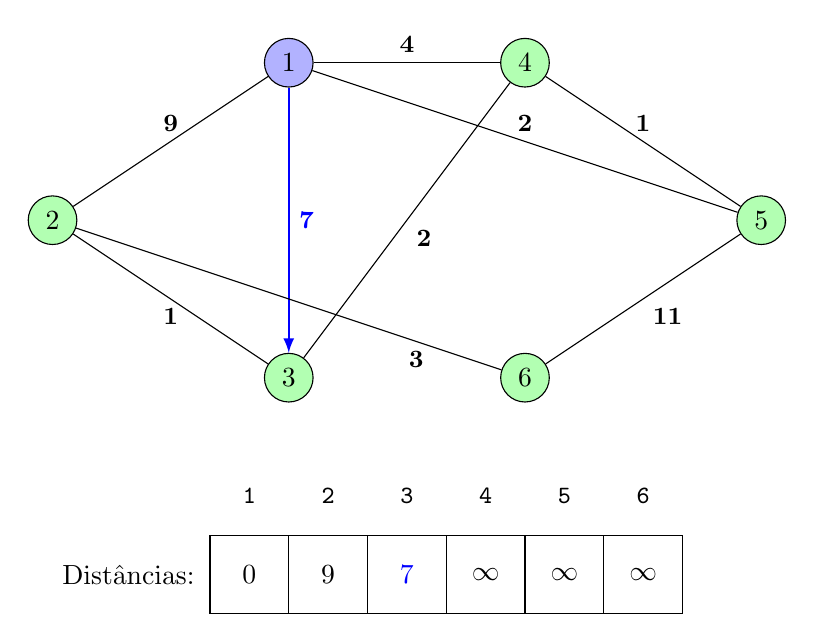
\begin{tikzpicture}
        \node[anchor=west] at (0, 0.5) { Distâncias: };

        \node[circle, draw, fill=blue!30] (a) at (3, 7) {1};
        \node[circle, draw, fill=green!30] (b) at (0, 5) {2};
        \node[circle, draw, fill=green!30] (c) at (3, 3) {3};
        \node[circle, draw, fill=green!30] (d) at (6, 7) {4};
        \node[circle, draw, fill=green!30] (e) at (9, 5) {5};
        \node[circle, draw, fill=green!30] (f) at (6, 3) {6};

        \draw (2, 0) grid (8, 1);

        \node at (2.5, 0.5) { $0$ };
        \node at (3.5, 0.5) { \textcolor{black}{$9$} };
        \node at (4.5, 0.5) { \textcolor{blue}{$7$} };
        \node at (5.5, 0.5) { $\infty$ };
        \node at (6.5, 0.5) { $\infty$ };
        \node at (7.5, 0.5) { $\infty$ };

        \node at (2.5, 1.5) { \small \texttt{1} };
        \node at (3.5, 1.5) { \small \texttt{2} };
        \node at (4.5, 1.5) { \small \texttt{3} };
        \node at (5.5, 1.5) { \small \texttt{4} };
        \node at (6.5, 1.5) { \small \texttt{5} };
        \node at (7.5, 1.5) { \small \texttt{6} };

        \draw (a) to node[midway,anchor=south] { \small \bfseries 9 } (b);
        %\draw (a) to node[midway,anchor=west] { \small \bfseries 7 } (c);
        \draw[-latex,thick,blue] (a) to node[midway,anchor=west] { \small \bfseries 7 } (c);
        \draw (a) to node[midway,anchor=south] { \small \bfseries 4 } (d);
        \draw (a) to node[midway,anchor=south] { \small \bfseries 2 } (e);
        \draw (b) to node[midway,anchor=north] { \small \bfseries 1 } (c);
        \draw (b) to node[pos=0.8,anchor=north] { \small \bfseries 3 } (f);
        \draw (c) to node[midway,anchor=north west] { \small \bfseries 2 } (d);
        \draw (d) to node[midway,anchor=south] { \small \bfseries 1 } (e);
        \draw (e) to node[midway,anchor=north west] { \small \bfseries 11 } (f);

    \end{tikzpicture}

\end{frame}

\begin{frame}[fragile]{Visualização do algoritmo de Bellman-Ford}

    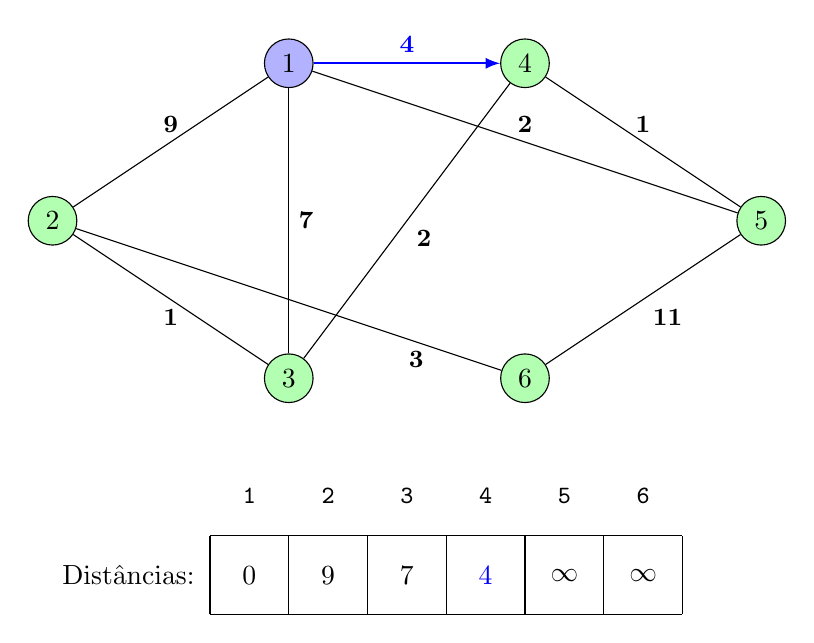
\begin{tikzpicture}
        \node[anchor=west] at (0, 0.5) { Distâncias: };

        \node[circle, draw, fill=blue!30] (a) at (3, 7) {1};
        \node[circle, draw, fill=green!30] (b) at (0, 5) {2};
        \node[circle, draw, fill=green!30] (c) at (3, 3) {3};
        \node[circle, draw, fill=green!30] (d) at (6, 7) {4};
        \node[circle, draw, fill=green!30] (e) at (9, 5) {5};
        \node[circle, draw, fill=green!30] (f) at (6, 3) {6};

        \draw (2, 0) grid (8, 1);

        \node at (2.5, 0.5) { $0$ };
        \node at (3.5, 0.5) { \textcolor{black}{$9$} };
        \node at (4.5, 0.5) { \textcolor{black}{$7$} };
        \node at (5.5, 0.5) { \textcolor{blue}{$4$} };
        \node at (6.5, 0.5) { $\infty$ };
        \node at (7.5, 0.5) { $\infty$ };

        \node at (2.5, 1.5) { \small \texttt{1} };
        \node at (3.5, 1.5) { \small \texttt{2} };
        \node at (4.5, 1.5) { \small \texttt{3} };
        \node at (5.5, 1.5) { \small \texttt{4} };
        \node at (6.5, 1.5) { \small \texttt{5} };
        \node at (7.5, 1.5) { \small \texttt{6} };

        \draw (a) to node[midway,anchor=south] { \small \bfseries 9 } (b);
        \draw (a) to node[midway,anchor=west] { \small \bfseries 7 } (c);
        %\draw (a) to node[midway,anchor=south] { \small \bfseries 4 } (d);
        \draw[-latex,thick,blue] (a) to node[midway,anchor=south] { \small \bfseries 4 } (d);
        \draw (a) to node[midway,anchor=south] { \small \bfseries 2 } (e);
        \draw (b) to node[midway,anchor=north] { \small \bfseries 1 } (c);
        \draw (b) to node[pos=0.8,anchor=north] { \small \bfseries 3 } (f);
        \draw (c) to node[midway,anchor=north west] { \small \bfseries 2 } (d);
        \draw (d) to node[midway,anchor=south] { \small \bfseries 1 } (e);
        \draw (e) to node[midway,anchor=north west] { \small \bfseries 11 } (f);

    \end{tikzpicture}

\end{frame}

\begin{frame}[fragile]{Visualização do algoritmo de Bellman-Ford}

    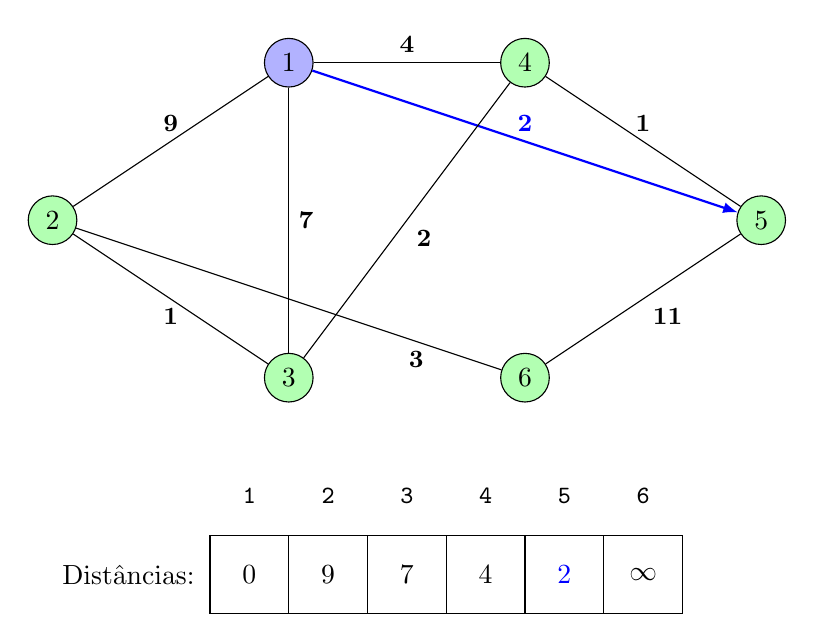
\begin{tikzpicture}
        \node[anchor=west] at (0, 0.5) { Distâncias: };

        \node[circle, draw, fill=blue!30] (a) at (3, 7) {1};
        \node[circle, draw, fill=green!30] (b) at (0, 5) {2};
        \node[circle, draw, fill=green!30] (c) at (3, 3) {3};
        \node[circle, draw, fill=green!30] (d) at (6, 7) {4};
        \node[circle, draw, fill=green!30] (e) at (9, 5) {5};
        \node[circle, draw, fill=green!30] (f) at (6, 3) {6};

        \draw (2, 0) grid (8, 1);

        \node at (2.5, 0.5) { $0$ };
        \node at (3.5, 0.5) { \textcolor{black}{$9$} };
        \node at (4.5, 0.5) { \textcolor{black}{$7$} };
        \node at (5.5, 0.5) { \textcolor{black}{$4$} };
        \node at (6.5, 0.5) { \textcolor{blue}{$2$} };
        \node at (7.5, 0.5) { $\infty$ };

        \node at (2.5, 1.5) { \small \texttt{1} };
        \node at (3.5, 1.5) { \small \texttt{2} };
        \node at (4.5, 1.5) { \small \texttt{3} };
        \node at (5.5, 1.5) { \small \texttt{4} };
        \node at (6.5, 1.5) { \small \texttt{5} };
        \node at (7.5, 1.5) { \small \texttt{6} };

        \draw (a) to node[midway,anchor=south] { \small \bfseries 9 } (b);
        \draw (a) to node[midway,anchor=west] { \small \bfseries 7 } (c);
        \draw (a) to node[midway,anchor=south] { \small \bfseries 4 } (d);
        %\draw (a) to node[midway,anchor=south] { \small \bfseries 2 } (e);
        \draw[-latex,thick,blue] (a) to node[midway,anchor=south] { \small \bfseries 2 } (e);
        \draw (b) to node[midway,anchor=north] { \small \bfseries 1 } (c);
        \draw (b) to node[pos=0.8,anchor=north] { \small \bfseries 3 } (f);
        \draw (c) to node[midway,anchor=north west] { \small \bfseries 2 } (d);
        \draw (d) to node[midway,anchor=south] { \small \bfseries 1 } (e);
        \draw (e) to node[midway,anchor=north west] { \small \bfseries 11 } (f);

    \end{tikzpicture}

\end{frame}

\begin{frame}[fragile]{Visualização do algoritmo de Bellman-Ford}

    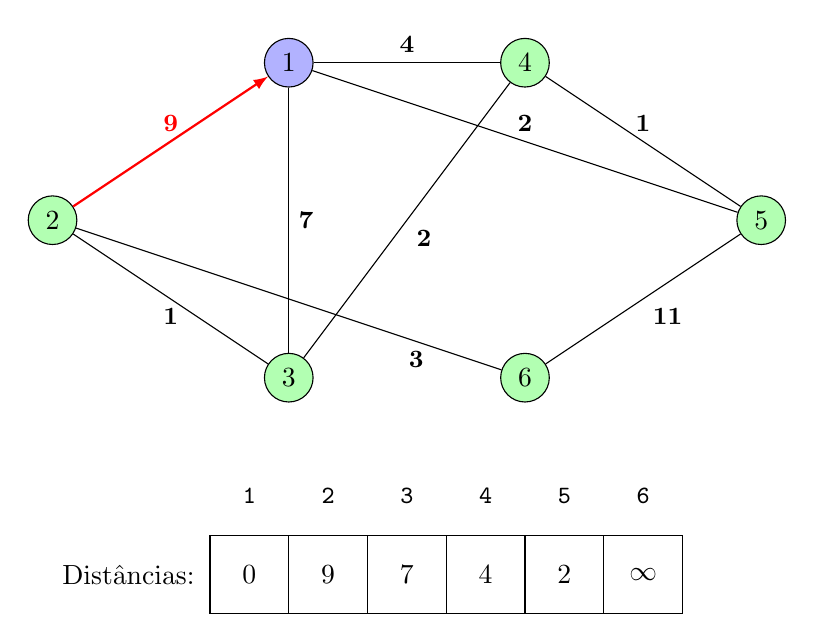
\begin{tikzpicture}
        \node[anchor=west] at (0, 0.5) { Distâncias: };

        \node[circle, draw, fill=blue!30] (a) at (3, 7) {1};
        \node[circle, draw, fill=green!30] (b) at (0, 5) {2};
        \node[circle, draw, fill=green!30] (c) at (3, 3) {3};
        \node[circle, draw, fill=green!30] (d) at (6, 7) {4};
        \node[circle, draw, fill=green!30] (e) at (9, 5) {5};
        \node[circle, draw, fill=green!30] (f) at (6, 3) {6};

        \draw (2, 0) grid (8, 1);

        \node at (2.5, 0.5) { $0$ };
        \node at (3.5, 0.5) { \textcolor{black}{$9$} };
        \node at (4.5, 0.5) { \textcolor{black}{$7$} };
        \node at (5.5, 0.5) { \textcolor{black}{$4$} };
        \node at (6.5, 0.5) { \textcolor{black}{$2$} };
        \node at (7.5, 0.5) { $\infty$ };

        \node at (2.5, 1.5) { \small \texttt{1} };
        \node at (3.5, 1.5) { \small \texttt{2} };
        \node at (4.5, 1.5) { \small \texttt{3} };
        \node at (5.5, 1.5) { \small \texttt{4} };
        \node at (6.5, 1.5) { \small \texttt{5} };
        \node at (7.5, 1.5) { \small \texttt{6} };

        \draw[latex-,thick,red] (a) to node[midway,anchor=south] { \small \bfseries 9 } (b);
        \draw (a) to node[midway,anchor=west] { \small \bfseries 7 } (c);
        \draw (a) to node[midway,anchor=south] { \small \bfseries 4 } (d);
        \draw (a) to node[midway,anchor=south] { \small \bfseries 2 } (e);
        \draw (b) to node[midway,anchor=north] { \small \bfseries 1 } (c);
        \draw (b) to node[pos=0.8,anchor=north] { \small \bfseries 3 } (f);
        \draw (c) to node[midway,anchor=north west] { \small \bfseries 2 } (d);
        \draw (d) to node[midway,anchor=south] { \small \bfseries 1 } (e);
        \draw (e) to node[midway,anchor=north west] { \small \bfseries 11 } (f);

    \end{tikzpicture}

\end{frame}

\begin{frame}[fragile]{Visualização do algoritmo de Bellman-Ford}

    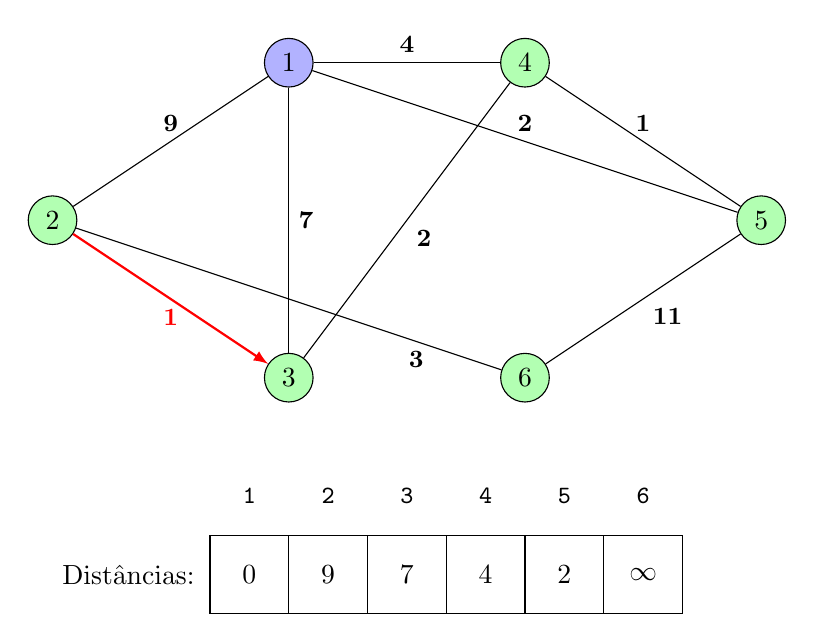
\begin{tikzpicture}
        \node[anchor=west] at (0, 0.5) { Distâncias: };

        \node[circle, draw, fill=blue!30] (a) at (3, 7) {1};
        \node[circle, draw, fill=green!30] (b) at (0, 5) {2};
        \node[circle, draw, fill=green!30] (c) at (3, 3) {3};
        \node[circle, draw, fill=green!30] (d) at (6, 7) {4};
        \node[circle, draw, fill=green!30] (e) at (9, 5) {5};
        \node[circle, draw, fill=green!30] (f) at (6, 3) {6};

        \draw (2, 0) grid (8, 1);

        \node at (2.5, 0.5) { $0$ };
        \node at (3.5, 0.5) { \textcolor{black}{$9$} };
        \node at (4.5, 0.5) { \textcolor{black}{$7$} };
        \node at (5.5, 0.5) { \textcolor{black}{$4$} };
        \node at (6.5, 0.5) { \textcolor{black}{$2$} };
        \node at (7.5, 0.5) { $\infty$ };

        \node at (2.5, 1.5) { \small \texttt{1} };
        \node at (3.5, 1.5) { \small \texttt{2} };
        \node at (4.5, 1.5) { \small \texttt{3} };
        \node at (5.5, 1.5) { \small \texttt{4} };
        \node at (6.5, 1.5) { \small \texttt{5} };
        \node at (7.5, 1.5) { \small \texttt{6} };

        \draw (a) to node[midway,anchor=south] { \small \bfseries 9 } (b);
        \draw (a) to node[midway,anchor=west] { \small \bfseries 7 } (c);
        \draw (a) to node[midway,anchor=south] { \small \bfseries 4 } (d);
        \draw (a) to node[midway,anchor=south] { \small \bfseries 2 } (e);
        %\draw (b) to node[midway,anchor=north] { \small \bfseries 1 } (c);
        \draw[-latex,thick,red] (b) to node[midway,anchor=north] { \small \bfseries 1 } (c);
        \draw (b) to node[pos=0.8,anchor=north] { \small \bfseries 3 } (f);
        \draw (c) to node[midway,anchor=north west] { \small \bfseries 2 } (d);
        \draw (d) to node[midway,anchor=south] { \small \bfseries 1 } (e);
        \draw (e) to node[midway,anchor=north west] { \small \bfseries 11 } (f);

    \end{tikzpicture}

\end{frame}

\begin{frame}[fragile]{Visualização do algoritmo de Bellman-Ford}

    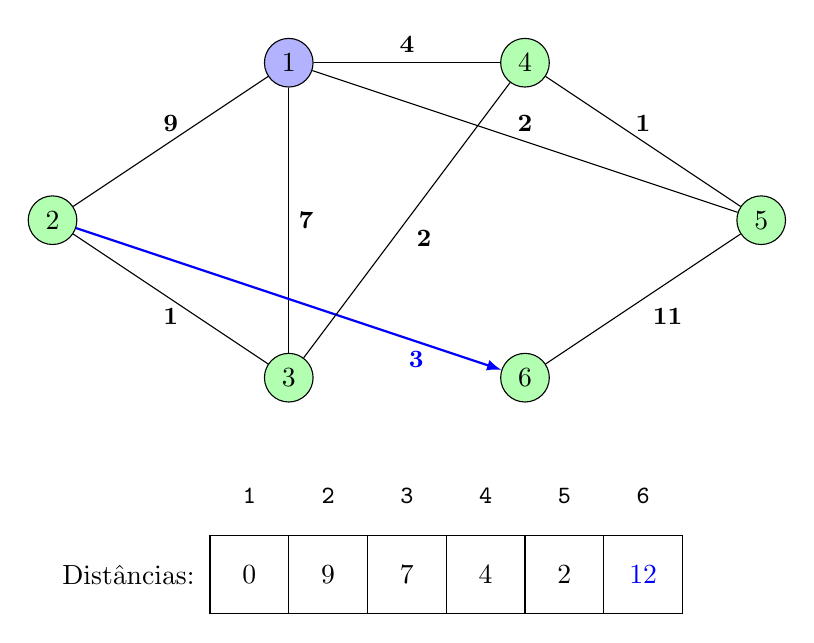
\begin{tikzpicture}
        \node[anchor=west] at (0, 0.5) { Distâncias: };

        \node[circle, draw, fill=blue!30] (a) at (3, 7) {1};
        \node[circle, draw, fill=green!30] (b) at (0, 5) {2};
        \node[circle, draw, fill=green!30] (c) at (3, 3) {3};
        \node[circle, draw, fill=green!30] (d) at (6, 7) {4};
        \node[circle, draw, fill=green!30] (e) at (9, 5) {5};
        \node[circle, draw, fill=green!30] (f) at (6, 3) {6};

        \draw (2, 0) grid (8, 1);

        \node at (2.5, 0.5) { $0$ };
        \node at (3.5, 0.5) { \textcolor{black}{$9$} };
        \node at (4.5, 0.5) { \textcolor{black}{$7$} };
        \node at (5.5, 0.5) { \textcolor{black}{$4$} };
        \node at (6.5, 0.5) { \textcolor{black}{$2$} };
        \node at (7.5, 0.5) { \textcolor{blue}{$12$} };

        \node at (2.5, 1.5) { \small \texttt{1} };
        \node at (3.5, 1.5) { \small \texttt{2} };
        \node at (4.5, 1.5) { \small \texttt{3} };
        \node at (5.5, 1.5) { \small \texttt{4} };
        \node at (6.5, 1.5) { \small \texttt{5} };
        \node at (7.5, 1.5) { \small \texttt{6} };

        \draw (a) to node[midway,anchor=south] { \small \bfseries 9 } (b);
        \draw (a) to node[midway,anchor=west] { \small \bfseries 7 } (c);
        \draw (a) to node[midway,anchor=south] { \small \bfseries 4 } (d);
        \draw (a) to node[midway,anchor=south] { \small \bfseries 2 } (e);
        \draw (b) to node[midway,anchor=north] { \small \bfseries 1 } (c);
        %\draw (b) to node[pos=0.8,anchor=north] { \small \bfseries 3 } (f);
        \draw[-latex,thick,blue] (b) to node[pos=0.8,anchor=north] { \small \bfseries 3 } (f);
        \draw (c) to node[midway,anchor=north west] { \small \bfseries 2 } (d);
        \draw (d) to node[midway,anchor=south] { \small \bfseries 1 } (e);
        \draw (e) to node[midway,anchor=north west] { \small \bfseries 11 } (f);

    \end{tikzpicture}

\end{frame}

\begin{frame}[fragile]{Visualização do algoritmo de Bellman-Ford}

    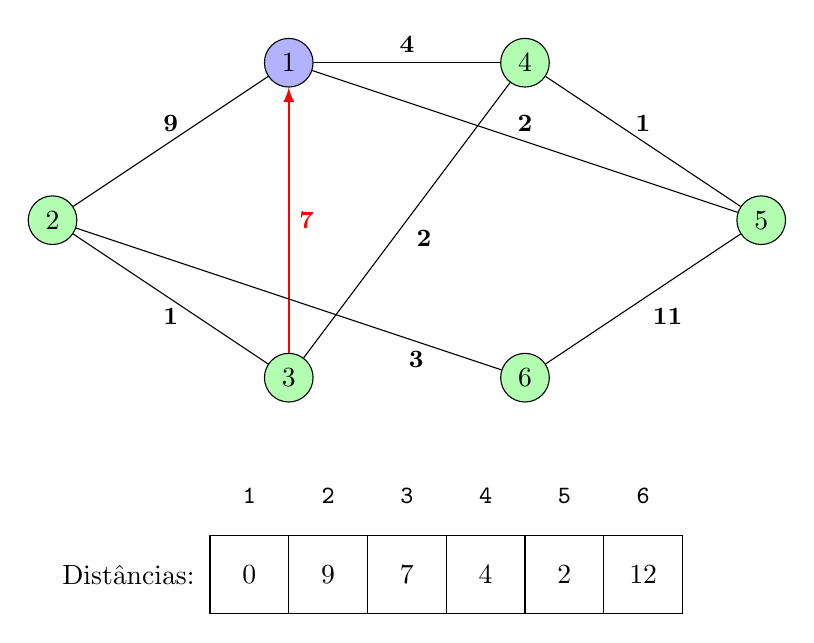
\begin{tikzpicture}
        \node[anchor=west] at (0, 0.5) { Distâncias: };

        \node[circle, draw, fill=blue!30] (a) at (3, 7) {1};
        \node[circle, draw, fill=green!30] (b) at (0, 5) {2};
        \node[circle, draw, fill=green!30] (c) at (3, 3) {3};
        \node[circle, draw, fill=green!30] (d) at (6, 7) {4};
        \node[circle, draw, fill=green!30] (e) at (9, 5) {5};
        \node[circle, draw, fill=green!30] (f) at (6, 3) {6};

        \draw (2, 0) grid (8, 1);

        \node at (2.5, 0.5) { $0$ };
        \node at (3.5, 0.5) { \textcolor{black}{$9$} };
        \node at (4.5, 0.5) { \textcolor{black}{$7$} };
        \node at (5.5, 0.5) { \textcolor{black}{$4$} };
        \node at (6.5, 0.5) { \textcolor{black}{$2$} };
        \node at (7.5, 0.5) { \textcolor{black}{$12$} };

        \node at (2.5, 1.5) { \small \texttt{1} };
        \node at (3.5, 1.5) { \small \texttt{2} };
        \node at (4.5, 1.5) { \small \texttt{3} };
        \node at (5.5, 1.5) { \small \texttt{4} };
        \node at (6.5, 1.5) { \small \texttt{5} };
        \node at (7.5, 1.5) { \small \texttt{6} };

        \draw (a) to node[midway,anchor=south] { \small \bfseries 9 } (b);
        %\draw (a) to node[midway,anchor=west] { \small \bfseries 7 } (c);
        \draw[latex-,thick,red] (a) to node[midway,anchor=west] { \small \bfseries 7 } (c);
        \draw (a) to node[midway,anchor=south] { \small \bfseries 4 } (d);
        \draw (a) to node[midway,anchor=south] { \small \bfseries 2 } (e);
        \draw (b) to node[midway,anchor=north] { \small \bfseries 1 } (c);
        \draw (b) to node[pos=0.8,anchor=north] { \small \bfseries 3 } (f);
        \draw (c) to node[midway,anchor=north west] { \small \bfseries 2 } (d);
        \draw (d) to node[midway,anchor=south] { \small \bfseries 1 } (e);
        \draw (e) to node[midway,anchor=north west] { \small \bfseries 11 } (f);

    \end{tikzpicture}

\end{frame}

\begin{frame}[fragile]{Visualização do algoritmo de Bellman-Ford}

    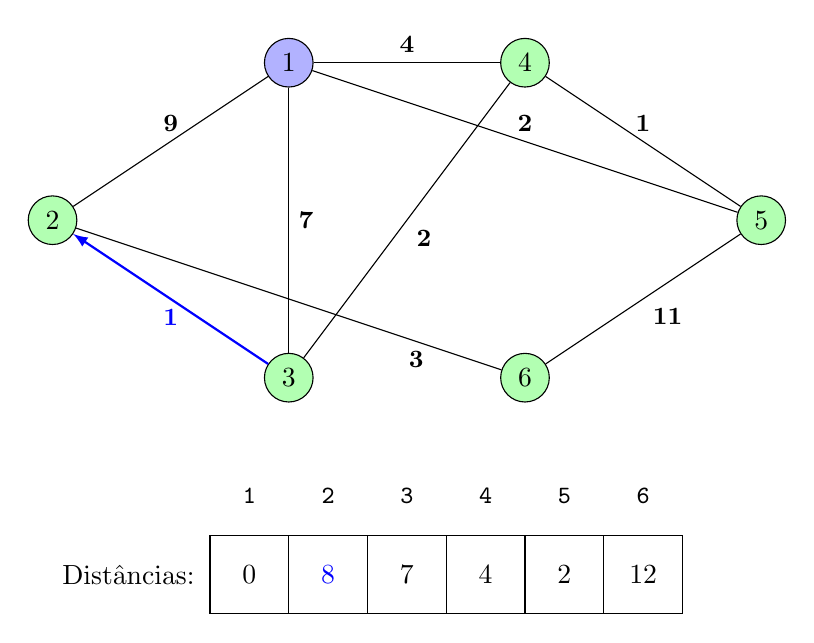
\begin{tikzpicture}
        \node[anchor=west] at (0, 0.5) { Distâncias: };

        \node[circle, draw, fill=blue!30] (a) at (3, 7) {1};
        \node[circle, draw, fill=green!30] (b) at (0, 5) {2};
        \node[circle, draw, fill=green!30] (c) at (3, 3) {3};
        \node[circle, draw, fill=green!30] (d) at (6, 7) {4};
        \node[circle, draw, fill=green!30] (e) at (9, 5) {5};
        \node[circle, draw, fill=green!30] (f) at (6, 3) {6};

        \draw (2, 0) grid (8, 1);

        \node at (2.5, 0.5) { $0$ };
        \node at (3.5, 0.5) { \textcolor{blue}{$8$} };
        \node at (4.5, 0.5) { \textcolor{black}{$7$} };
        \node at (5.5, 0.5) { \textcolor{black}{$4$} };
        \node at (6.5, 0.5) { \textcolor{black}{$2$} };
        \node at (7.5, 0.5) { \textcolor{black}{$12$} };

        \node at (2.5, 1.5) { \small \texttt{1} };
        \node at (3.5, 1.5) { \small \texttt{2} };
        \node at (4.5, 1.5) { \small \texttt{3} };
        \node at (5.5, 1.5) { \small \texttt{4} };
        \node at (6.5, 1.5) { \small \texttt{5} };
        \node at (7.5, 1.5) { \small \texttt{6} };

        \draw (a) to node[midway,anchor=south] { \small \bfseries 9 } (b);
        \draw (a) to node[midway,anchor=west] { \small \bfseries 7 } (c);
        \draw (a) to node[midway,anchor=south] { \small \bfseries 4 } (d);
        \draw (a) to node[midway,anchor=south] { \small \bfseries 2 } (e);
        %\draw (b) to node[midway,anchor=north] { \small \bfseries 1 } (c);
        \draw[latex-,thick,blue] (b) to node[midway,anchor=north] { \small \bfseries 1 } (c);
        \draw (b) to node[pos=0.8,anchor=north] { \small \bfseries 3 } (f);
        \draw (c) to node[midway,anchor=north west] { \small \bfseries 2 } (d);
        \draw (d) to node[midway,anchor=south] { \small \bfseries 1 } (e);
        \draw (e) to node[midway,anchor=north west] { \small \bfseries 11 } (f);

    \end{tikzpicture}

\end{frame}

\begin{frame}[fragile]{Visualização do algoritmo de Bellman-Ford}

    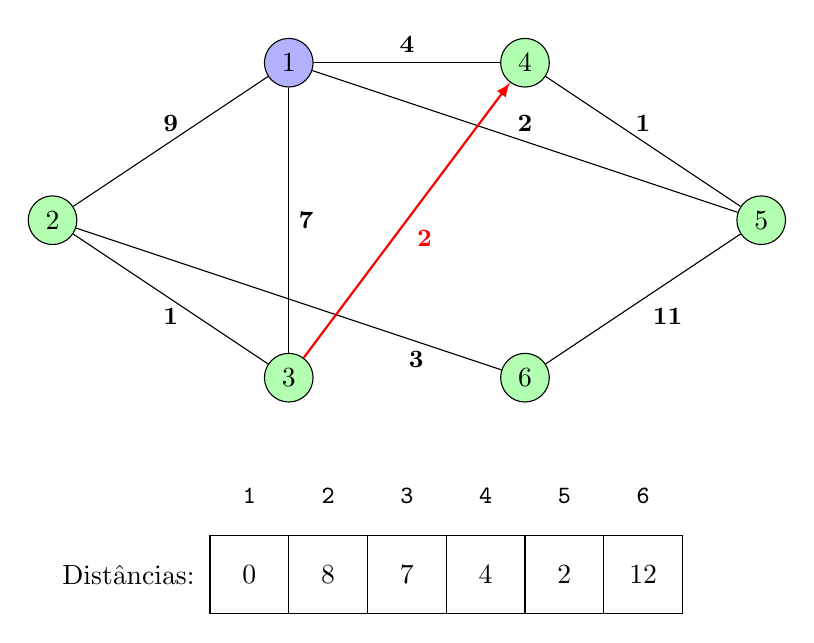
\begin{tikzpicture}
        \node[anchor=west] at (0, 0.5) { Distâncias: };

        \node[circle, draw, fill=blue!30] (a) at (3, 7) {1};
        \node[circle, draw, fill=green!30] (b) at (0, 5) {2};
        \node[circle, draw, fill=green!30] (c) at (3, 3) {3};
        \node[circle, draw, fill=green!30] (d) at (6, 7) {4};
        \node[circle, draw, fill=green!30] (e) at (9, 5) {5};
        \node[circle, draw, fill=green!30] (f) at (6, 3) {6};

        \draw (2, 0) grid (8, 1);

        \node at (2.5, 0.5) { $0$ };
        \node at (3.5, 0.5) { \textcolor{black}{$8$} };
        \node at (4.5, 0.5) { \textcolor{black}{$7$} };
        \node at (5.5, 0.5) { \textcolor{black}{$4$} };
        \node at (6.5, 0.5) { \textcolor{black}{$2$} };
        \node at (7.5, 0.5) { \textcolor{black}{$12$} };

        \node at (2.5, 1.5) { \small \texttt{1} };
        \node at (3.5, 1.5) { \small \texttt{2} };
        \node at (4.5, 1.5) { \small \texttt{3} };
        \node at (5.5, 1.5) { \small \texttt{4} };
        \node at (6.5, 1.5) { \small \texttt{5} };
        \node at (7.5, 1.5) { \small \texttt{6} };

        \draw (a) to node[midway,anchor=south] { \small \bfseries 9 } (b);
        \draw (a) to node[midway,anchor=west] { \small \bfseries 7 } (c);
        \draw (a) to node[midway,anchor=south] { \small \bfseries 4 } (d);
        \draw (a) to node[midway,anchor=south] { \small \bfseries 2 } (e);
        \draw (b) to node[midway,anchor=north] { \small \bfseries 1 } (c);
        \draw (b) to node[pos=0.8,anchor=north] { \small \bfseries 3 } (f);
        %\draw (c) to node[midway,anchor=north west] { \small \bfseries 2 } (d);
        \draw[-latex,thick,red] (c) to node[midway,anchor=north west] { \small \bfseries 2 } (d);
        \draw (d) to node[midway,anchor=south] { \small \bfseries 1 } (e);
        \draw (e) to node[midway,anchor=north west] { \small \bfseries 11 } (f);

    \end{tikzpicture}

\end{frame}

\begin{frame}[fragile]{Visualização do algoritmo de Bellman-Ford}

    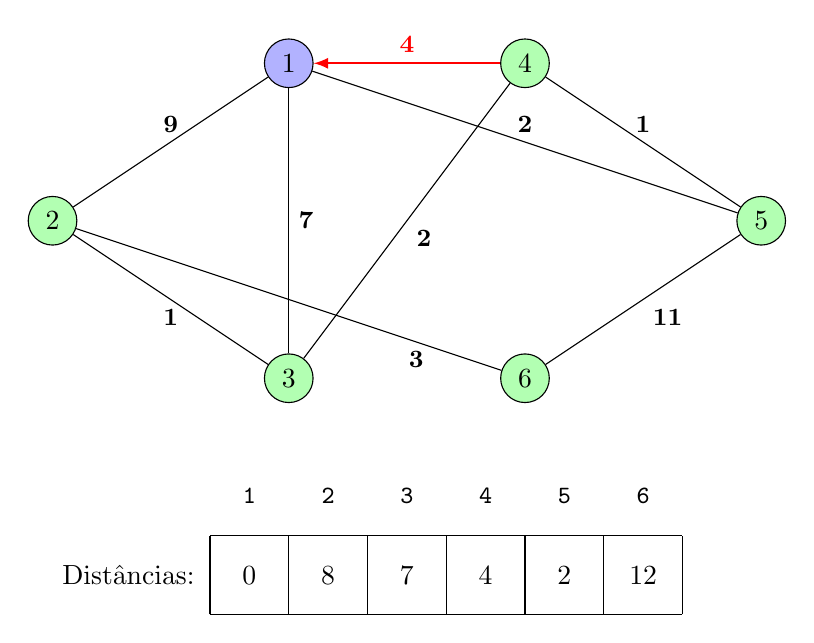
\begin{tikzpicture}
        \node[anchor=west] at (0, 0.5) { Distâncias: };

        \node[circle, draw, fill=blue!30] (a) at (3, 7) {1};
        \node[circle, draw, fill=green!30] (b) at (0, 5) {2};
        \node[circle, draw, fill=green!30] (c) at (3, 3) {3};
        \node[circle, draw, fill=green!30] (d) at (6, 7) {4};
        \node[circle, draw, fill=green!30] (e) at (9, 5) {5};
        \node[circle, draw, fill=green!30] (f) at (6, 3) {6};

        \draw (2, 0) grid (8, 1);

        \node at (2.5, 0.5) { $0$ };
        \node at (3.5, 0.5) { \textcolor{black}{$8$} };
        \node at (4.5, 0.5) { \textcolor{black}{$7$} };
        \node at (5.5, 0.5) { \textcolor{black}{$4$} };
        \node at (6.5, 0.5) { \textcolor{black}{$2$} };
        \node at (7.5, 0.5) { \textcolor{black}{$12$} };

        \node at (2.5, 1.5) { \small \texttt{1} };
        \node at (3.5, 1.5) { \small \texttt{2} };
        \node at (4.5, 1.5) { \small \texttt{3} };
        \node at (5.5, 1.5) { \small \texttt{4} };
        \node at (6.5, 1.5) { \small \texttt{5} };
        \node at (7.5, 1.5) { \small \texttt{6} };

        \draw (a) to node[midway,anchor=south] { \small \bfseries 9 } (b);
        \draw (a) to node[midway,anchor=west] { \small \bfseries 7 } (c);
        %\draw (a) to node[midway,anchor=south] { \small \bfseries 4 } (d);
        \draw[latex-,thick,red] (a) to node[midway,anchor=south] { \small \bfseries 4 } (d);
        \draw (a) to node[midway,anchor=south] { \small \bfseries 2 } (e);
        \draw (b) to node[midway,anchor=north] { \small \bfseries 1 } (c);
        \draw (b) to node[pos=0.8,anchor=north] { \small \bfseries 3 } (f);
        \draw (c) to node[midway,anchor=north west] { \small \bfseries 2 } (d);
        \draw (d) to node[midway,anchor=south] { \small \bfseries 1 } (e);
        \draw (e) to node[midway,anchor=north west] { \small \bfseries 11 } (f);

    \end{tikzpicture}

\end{frame}

\begin{frame}[fragile]{Visualização do algoritmo de Bellman-Ford}

    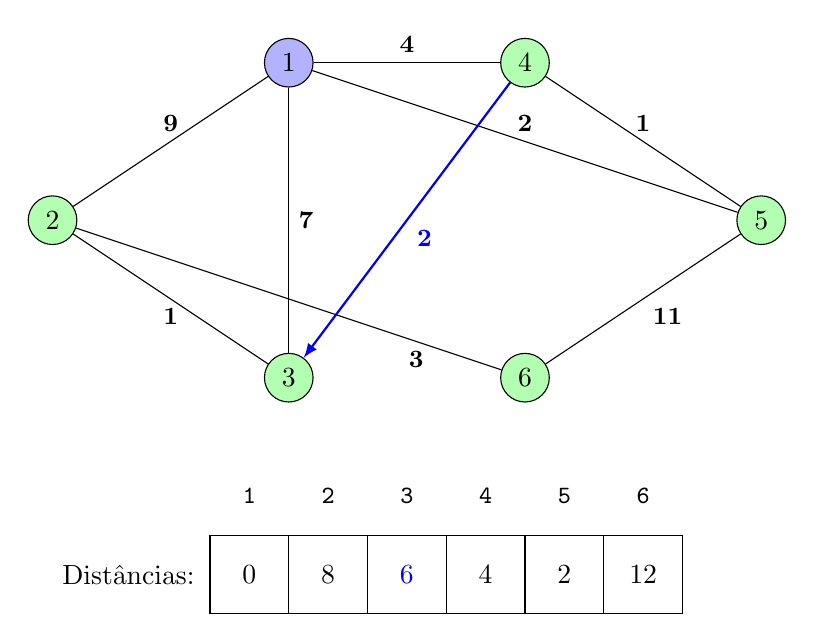
\begin{tikzpicture}
        \node[anchor=west] at (0, 0.5) { Distâncias: };

        \node[circle, draw, fill=blue!30] (a) at (3, 7) {1};
        \node[circle, draw, fill=green!30] (b) at (0, 5) {2};
        \node[circle, draw, fill=green!30] (c) at (3, 3) {3};
        \node[circle, draw, fill=green!30] (d) at (6, 7) {4};
        \node[circle, draw, fill=green!30] (e) at (9, 5) {5};
        \node[circle, draw, fill=green!30] (f) at (6, 3) {6};

        \draw (2, 0) grid (8, 1);

        \node at (2.5, 0.5) { $0$ };
        \node at (3.5, 0.5) { \textcolor{black}{$8$} };
        \node at (4.5, 0.5) { \textcolor{blue}{$6$} };
        \node at (5.5, 0.5) { \textcolor{black}{$4$} };
        \node at (6.5, 0.5) { \textcolor{black}{$2$} };
        \node at (7.5, 0.5) { \textcolor{black}{$12$} };

        \node at (2.5, 1.5) { \small \texttt{1} };
        \node at (3.5, 1.5) { \small \texttt{2} };
        \node at (4.5, 1.5) { \small \texttt{3} };
        \node at (5.5, 1.5) { \small \texttt{4} };
        \node at (6.5, 1.5) { \small \texttt{5} };
        \node at (7.5, 1.5) { \small \texttt{6} };

        \draw (a) to node[midway,anchor=south] { \small \bfseries 9 } (b);
        \draw (a) to node[midway,anchor=west] { \small \bfseries 7 } (c);
        \draw (a) to node[midway,anchor=south] { \small \bfseries 4 } (d);
        \draw (a) to node[midway,anchor=south] { \small \bfseries 2 } (e);
        \draw (b) to node[midway,anchor=north] { \small \bfseries 1 } (c);
        \draw (b) to node[pos=0.8,anchor=north] { \small \bfseries 3 } (f);
        \draw[latex-,thick,blue] (c) to node[midway,anchor=north west] { \small \bfseries 2 } (d);
        \draw (d) to node[midway,anchor=south] { \small \bfseries 1 } (e);
        \draw (e) to node[midway,anchor=north west] { \small \bfseries 11 } (f);

    \end{tikzpicture}

\end{frame}



\begin{frame}[fragile]{Visualização do algoritmo de Bellman-Ford}

    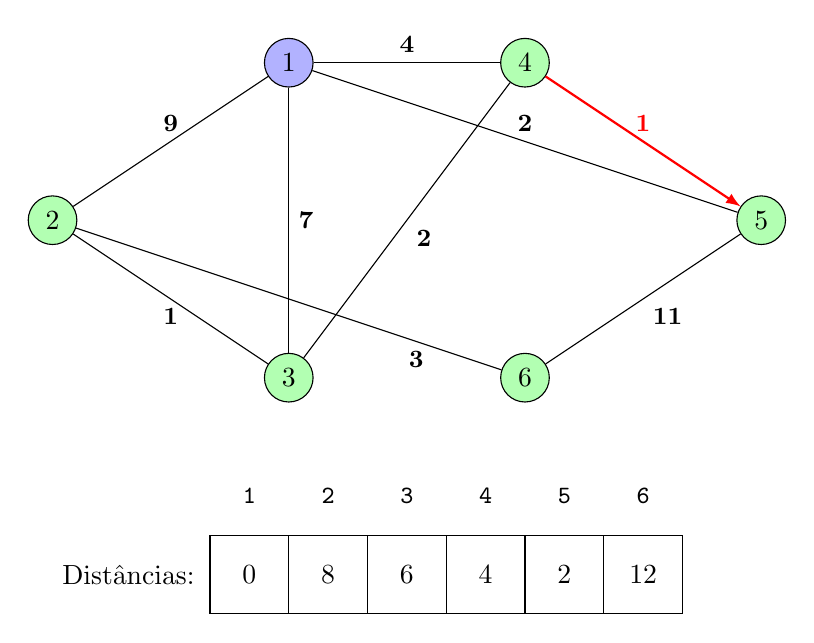
\begin{tikzpicture}
        \node[anchor=west] at (0, 0.5) { Distâncias: };

        \node[circle, draw, fill=blue!30] (a) at (3, 7) {1};
        \node[circle, draw, fill=green!30] (b) at (0, 5) {2};
        \node[circle, draw, fill=green!30] (c) at (3, 3) {3};
        \node[circle, draw, fill=green!30] (d) at (6, 7) {4};
        \node[circle, draw, fill=green!30] (e) at (9, 5) {5};
        \node[circle, draw, fill=green!30] (f) at (6, 3) {6};

        \draw (2, 0) grid (8, 1);

        \node at (2.5, 0.5) { $0$ };
        \node at (3.5, 0.5) { \textcolor{black}{$8$} };
        \node at (4.5, 0.5) { \textcolor{black}{$6$} };
        \node at (5.5, 0.5) { \textcolor{black}{$4$} };
        \node at (6.5, 0.5) { \textcolor{black}{$2$} };
        \node at (7.5, 0.5) { \textcolor{black}{$12$} };

        \node at (2.5, 1.5) { \small \texttt{1} };
        \node at (3.5, 1.5) { \small \texttt{2} };
        \node at (4.5, 1.5) { \small \texttt{3} };
        \node at (5.5, 1.5) { \small \texttt{4} };
        \node at (6.5, 1.5) { \small \texttt{5} };
        \node at (7.5, 1.5) { \small \texttt{6} };

        \draw (a) to node[midway,anchor=south] { \small \bfseries 9 } (b);
        \draw (a) to node[midway,anchor=west] { \small \bfseries 7 } (c);
        \draw (a) to node[midway,anchor=south] { \small \bfseries 4 } (d);
        \draw (a) to node[midway,anchor=south] { \small \bfseries 2 } (e);
        \draw (b) to node[midway,anchor=north] { \small \bfseries 1 } (c);
        \draw (b) to node[pos=0.8,anchor=north] { \small \bfseries 3 } (f);
        \draw (c) to node[midway,anchor=north west] { \small \bfseries 2 } (d);
        %\draw (d) to node[midway,anchor=south] { \small \bfseries 1 } (e);
        \draw[-latex,thick,red] (d) to node[midway,anchor=south] { \small \bfseries 1 } (e);
        \draw (e) to node[midway,anchor=north west] { \small \bfseries 11 } (f);

    \end{tikzpicture}

\end{frame}

\begin{frame}[fragile]{Visualização do algoritmo de Bellman-Ford}

    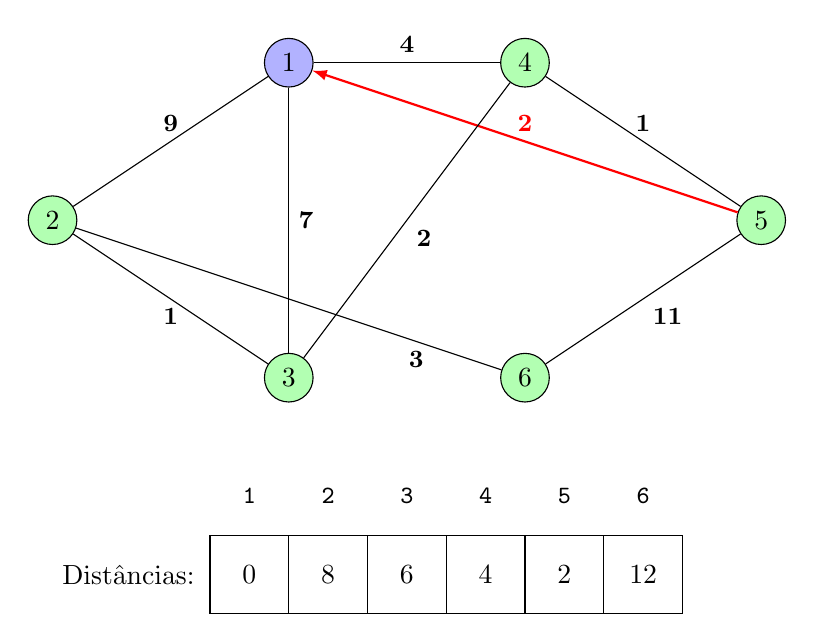
\begin{tikzpicture}
        \node[anchor=west] at (0, 0.5) { Distâncias: };

        \node[circle, draw, fill=blue!30] (a) at (3, 7) {1};
        \node[circle, draw, fill=green!30] (b) at (0, 5) {2};
        \node[circle, draw, fill=green!30] (c) at (3, 3) {3};
        \node[circle, draw, fill=green!30] (d) at (6, 7) {4};
        \node[circle, draw, fill=green!30] (e) at (9, 5) {5};
        \node[circle, draw, fill=green!30] (f) at (6, 3) {6};

        \draw (2, 0) grid (8, 1);

        \node at (2.5, 0.5) { $0$ };
        \node at (3.5, 0.5) { \textcolor{black}{$8$} };
        \node at (4.5, 0.5) { \textcolor{black}{$6$} };
        \node at (5.5, 0.5) { \textcolor{black}{$4$} };
        \node at (6.5, 0.5) { \textcolor{black}{$2$} };
        \node at (7.5, 0.5) { \textcolor{black}{$12$} };

        \node at (2.5, 1.5) { \small \texttt{1} };
        \node at (3.5, 1.5) { \small \texttt{2} };
        \node at (4.5, 1.5) { \small \texttt{3} };
        \node at (5.5, 1.5) { \small \texttt{4} };
        \node at (6.5, 1.5) { \small \texttt{5} };
        \node at (7.5, 1.5) { \small \texttt{6} };

        \draw (a) to node[midway,anchor=south] { \small \bfseries 9 } (b);
        \draw (a) to node[midway,anchor=west] { \small \bfseries 7 } (c);
        \draw (a) to node[midway,anchor=south] { \small \bfseries 4 } (d);
        %\draw (a) to node[midway,anchor=south] { \small \bfseries 2 } (e);
        \draw[latex-,thick,red] (a) to node[midway,anchor=south] { \small \bfseries 2 } (e);
        \draw (b) to node[midway,anchor=north] { \small \bfseries 1 } (c);
        \draw (b) to node[pos=0.8,anchor=north] { \small \bfseries 3 } (f);
        \draw (c) to node[midway,anchor=north west] { \small \bfseries 2 } (d);
        \draw (d) to node[midway,anchor=south] { \small \bfseries 1 } (e);
        \draw (e) to node[midway,anchor=north west] { \small \bfseries 11 } (f);

    \end{tikzpicture}

\end{frame}

\begin{frame}[fragile]{Visualização do algoritmo de Bellman-Ford}

    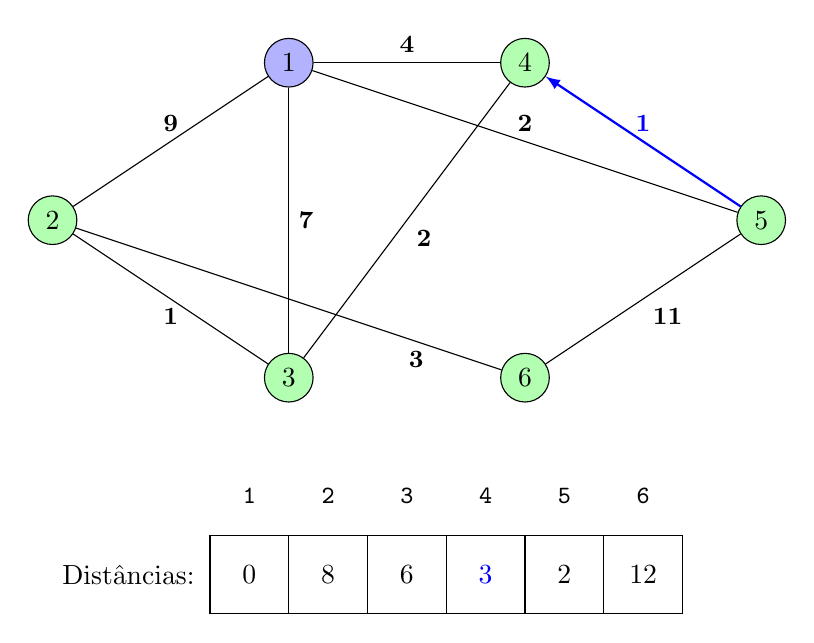
\begin{tikzpicture}
        \node[anchor=west] at (0, 0.5) { Distâncias: };

        \node[circle, draw, fill=blue!30] (a) at (3, 7) {1};
        \node[circle, draw, fill=green!30] (b) at (0, 5) {2};
        \node[circle, draw, fill=green!30] (c) at (3, 3) {3};
        \node[circle, draw, fill=green!30] (d) at (6, 7) {4};
        \node[circle, draw, fill=green!30] (e) at (9, 5) {5};
        \node[circle, draw, fill=green!30] (f) at (6, 3) {6};

        \draw (2, 0) grid (8, 1);

        \node at (2.5, 0.5) { $0$ };
        \node at (3.5, 0.5) { \textcolor{black}{$8$} };
        \node at (4.5, 0.5) { \textcolor{black}{$6$} };
        \node at (5.5, 0.5) { \textcolor{blue}{$3$} };
        \node at (6.5, 0.5) { \textcolor{black}{$2$} };
        \node at (7.5, 0.5) { \textcolor{black}{$12$} };

        \node at (2.5, 1.5) { \small \texttt{1} };
        \node at (3.5, 1.5) { \small \texttt{2} };
        \node at (4.5, 1.5) { \small \texttt{3} };
        \node at (5.5, 1.5) { \small \texttt{4} };
        \node at (6.5, 1.5) { \small \texttt{5} };
        \node at (7.5, 1.5) { \small \texttt{6} };

        \draw (a) to node[midway,anchor=south] { \small \bfseries 9 } (b);
        \draw (a) to node[midway,anchor=west] { \small \bfseries 7 } (c);
        \draw (a) to node[midway,anchor=south] { \small \bfseries 4 } (d);
        \draw (a) to node[midway,anchor=south] { \small \bfseries 2 } (e);
        \draw (b) to node[midway,anchor=north] { \small \bfseries 1 } (c);
        \draw (b) to node[pos=0.8,anchor=north] { \small \bfseries 3 } (f);
        \draw (c) to node[midway,anchor=north west] { \small \bfseries 2 } (d);
        %\draw (d) to node[midway,anchor=south] { \small \bfseries 1 } (e);
        \draw[latex-,thick,blue] (d) to node[midway,anchor=south] { \small \bfseries 1 } (e);
        \draw (e) to node[midway,anchor=north west] { \small \bfseries 11 } (f);

    \end{tikzpicture}

\end{frame}

\begin{frame}[fragile]{Visualização do algoritmo de Bellman-Ford}

    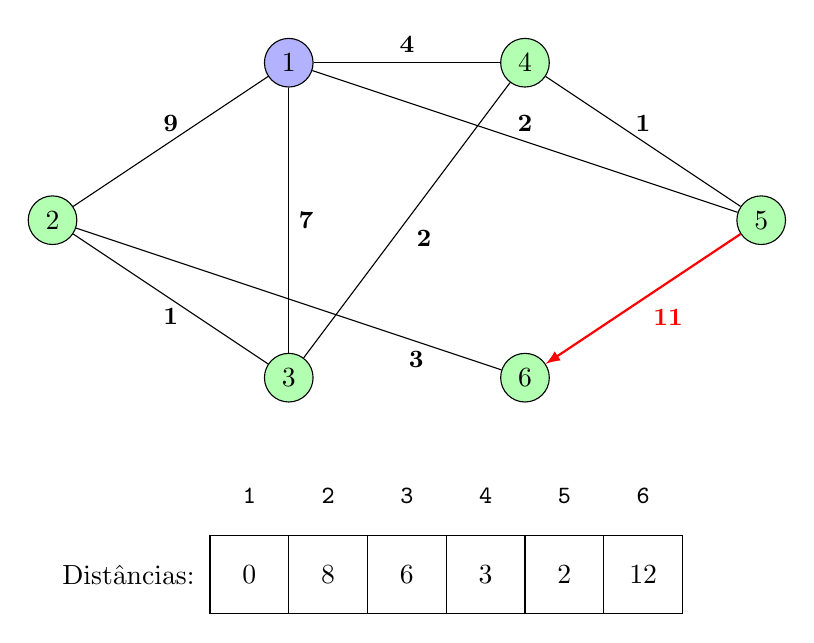
\begin{tikzpicture}
        \node[anchor=west] at (0, 0.5) { Distâncias: };

        \node[circle, draw, fill=blue!30] (a) at (3, 7) {1};
        \node[circle, draw, fill=green!30] (b) at (0, 5) {2};
        \node[circle, draw, fill=green!30] (c) at (3, 3) {3};
        \node[circle, draw, fill=green!30] (d) at (6, 7) {4};
        \node[circle, draw, fill=green!30] (e) at (9, 5) {5};
        \node[circle, draw, fill=green!30] (f) at (6, 3) {6};

        \draw (2, 0) grid (8, 1);

        \node at (2.5, 0.5) { $0$ };
        \node at (3.5, 0.5) { \textcolor{black}{$8$} };
        \node at (4.5, 0.5) { \textcolor{black}{$6$} };
        \node at (5.5, 0.5) { \textcolor{black}{$3$} };
        \node at (6.5, 0.5) { \textcolor{black}{$2$} };
        \node at (7.5, 0.5) { \textcolor{black}{$12$} };

        \node at (2.5, 1.5) { \small \texttt{1} };
        \node at (3.5, 1.5) { \small \texttt{2} };
        \node at (4.5, 1.5) { \small \texttt{3} };
        \node at (5.5, 1.5) { \small \texttt{4} };
        \node at (6.5, 1.5) { \small \texttt{5} };
        \node at (7.5, 1.5) { \small \texttt{6} };

        \draw (a) to node[midway,anchor=south] { \small \bfseries 9 } (b);
        \draw (a) to node[midway,anchor=west] { \small \bfseries 7 } (c);
        \draw (a) to node[midway,anchor=south] { \small \bfseries 4 } (d);
        \draw (a) to node[midway,anchor=south] { \small \bfseries 2 } (e);
        \draw (b) to node[midway,anchor=north] { \small \bfseries 1 } (c);
        \draw (b) to node[pos=0.8,anchor=north] { \small \bfseries 3 } (f);
        \draw (c) to node[midway,anchor=north west] { \small \bfseries 2 } (d);
        \draw (d) to node[midway,anchor=south] { \small \bfseries 1 } (e);
        %\draw (e) to node[midway,anchor=north west] { \small \bfseries 11 } (f);
        \draw[-latex,thick,red] (e) to node[midway,anchor=north west] { \small \bfseries 11 } (f);

    \end{tikzpicture}

\end{frame}


\begin{frame}[fragile]{Visualização do algoritmo de Bellman-Ford}

    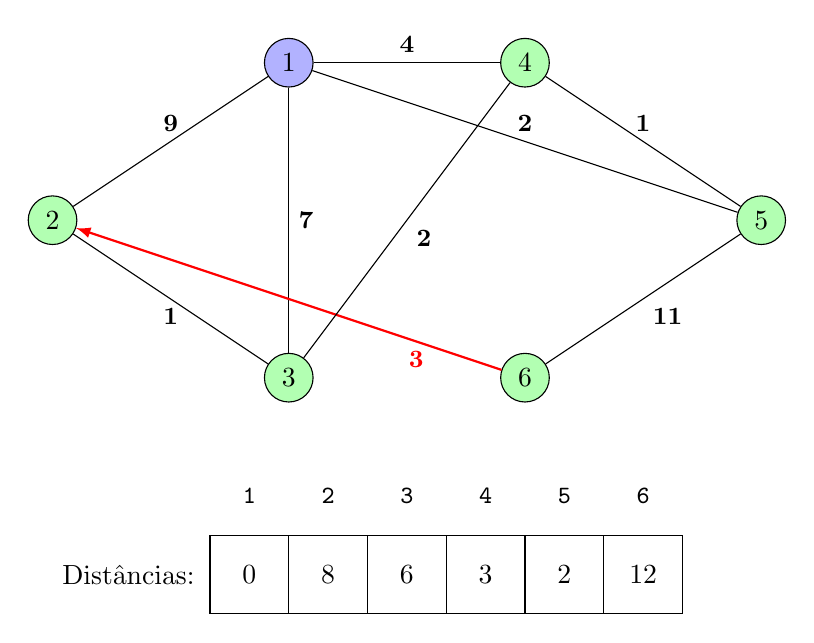
\begin{tikzpicture}
        \node[anchor=west] at (0, 0.5) { Distâncias: };

        \node[circle, draw, fill=blue!30] (a) at (3, 7) {1};
        \node[circle, draw, fill=green!30] (b) at (0, 5) {2};
        \node[circle, draw, fill=green!30] (c) at (3, 3) {3};
        \node[circle, draw, fill=green!30] (d) at (6, 7) {4};
        \node[circle, draw, fill=green!30] (e) at (9, 5) {5};
        \node[circle, draw, fill=green!30] (f) at (6, 3) {6};

        \draw (2, 0) grid (8, 1);

        \node at (2.5, 0.5) { $0$ };
        \node at (3.5, 0.5) { \textcolor{black}{$8$} };
        \node at (4.5, 0.5) { \textcolor{black}{$6$} };
        \node at (5.5, 0.5) { \textcolor{black}{$3$} };
        \node at (6.5, 0.5) { \textcolor{black}{$2$} };
        \node at (7.5, 0.5) { \textcolor{black}{$12$} };

        \node at (2.5, 1.5) { \small \texttt{1} };
        \node at (3.5, 1.5) { \small \texttt{2} };
        \node at (4.5, 1.5) { \small \texttt{3} };
        \node at (5.5, 1.5) { \small \texttt{4} };
        \node at (6.5, 1.5) { \small \texttt{5} };
        \node at (7.5, 1.5) { \small \texttt{6} };

        \draw (a) to node[midway,anchor=south] { \small \bfseries 9 } (b);
        \draw (a) to node[midway,anchor=west] { \small \bfseries 7 } (c);
        \draw (a) to node[midway,anchor=south] { \small \bfseries 4 } (d);
        \draw (a) to node[midway,anchor=south] { \small \bfseries 2 } (e);
        \draw (b) to node[midway,anchor=north] { \small \bfseries 1 } (c);
        %\draw (b) to node[pos=0.8,anchor=north] { \small \bfseries 3 } (f);
        \draw[latex-,thick,red] (b) to node[pos=0.8,anchor=north] { \small \bfseries 3 } (f);
        \draw (c) to node[midway,anchor=north west] { \small \bfseries 2 } (d);
        \draw (d) to node[midway,anchor=south] { \small \bfseries 1 } (e);
        \draw (e) to node[midway,anchor=north west] { \small \bfseries 11 } (f);

    \end{tikzpicture}

\end{frame}

\begin{frame}[fragile]{Visualização do algoritmo de Bellman-Ford}

    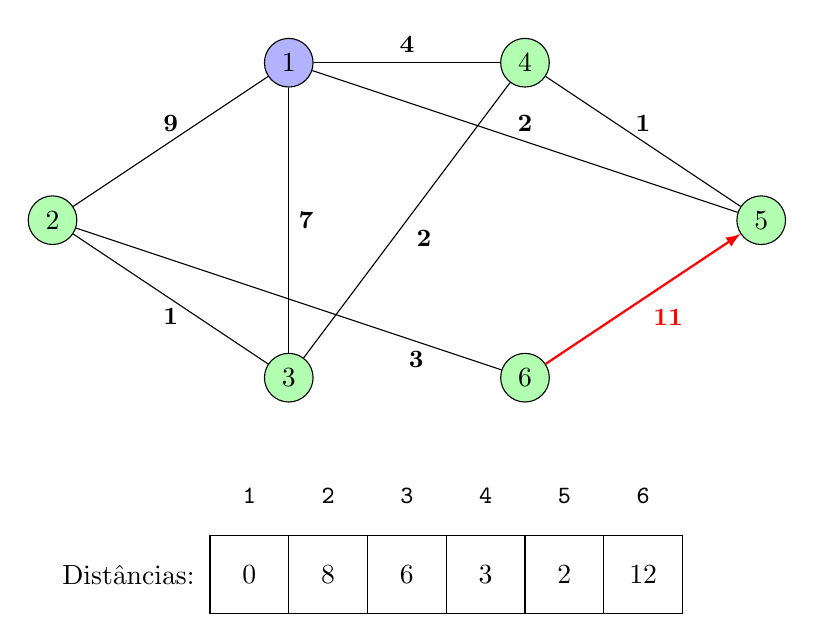
\begin{tikzpicture}
        \node[anchor=west] at (0, 0.5) { Distâncias: };

        \node[circle, draw, fill=blue!30] (a) at (3, 7) {1};
        \node[circle, draw, fill=green!30] (b) at (0, 5) {2};
        \node[circle, draw, fill=green!30] (c) at (3, 3) {3};
        \node[circle, draw, fill=green!30] (d) at (6, 7) {4};
        \node[circle, draw, fill=green!30] (e) at (9, 5) {5};
        \node[circle, draw, fill=green!30] (f) at (6, 3) {6};

        \draw (2, 0) grid (8, 1);

        \node at (2.5, 0.5) { $0$ };
        \node at (3.5, 0.5) { \textcolor{black}{$8$} };
        \node at (4.5, 0.5) { \textcolor{black}{$6$} };
        \node at (5.5, 0.5) { \textcolor{black}{$3$} };
        \node at (6.5, 0.5) { \textcolor{black}{$2$} };
        \node at (7.5, 0.5) { \textcolor{black}{$12$} };

        \node at (2.5, 1.5) { \small \texttt{1} };
        \node at (3.5, 1.5) { \small \texttt{2} };
        \node at (4.5, 1.5) { \small \texttt{3} };
        \node at (5.5, 1.5) { \small \texttt{4} };
        \node at (6.5, 1.5) { \small \texttt{5} };
        \node at (7.5, 1.5) { \small \texttt{6} };

        \draw (a) to node[midway,anchor=south] { \small \bfseries 9 } (b);
        \draw (a) to node[midway,anchor=west] { \small \bfseries 7 } (c);
        \draw (a) to node[midway,anchor=south] { \small \bfseries 4 } (d);
        \draw (a) to node[midway,anchor=south] { \small \bfseries 2 } (e);
        \draw (b) to node[midway,anchor=north] { \small \bfseries 1 } (c);
        \draw (b) to node[pos=0.8,anchor=north] { \small \bfseries 3 } (f);
        \draw (c) to node[midway,anchor=north west] { \small \bfseries 2 } (d);
        \draw (d) to node[midway,anchor=south] { \small \bfseries 1 } (e);
        %\draw (e) to node[midway,anchor=north west] { \small \bfseries 11 } (f);
        \draw[latex-,thick,red] (e) to node[midway,anchor=north west] { \small \bfseries 11 } (f);

    \end{tikzpicture}

\end{frame}

\begin{frame}[fragile]{Visualização do algoritmo de Bellman-Ford}

    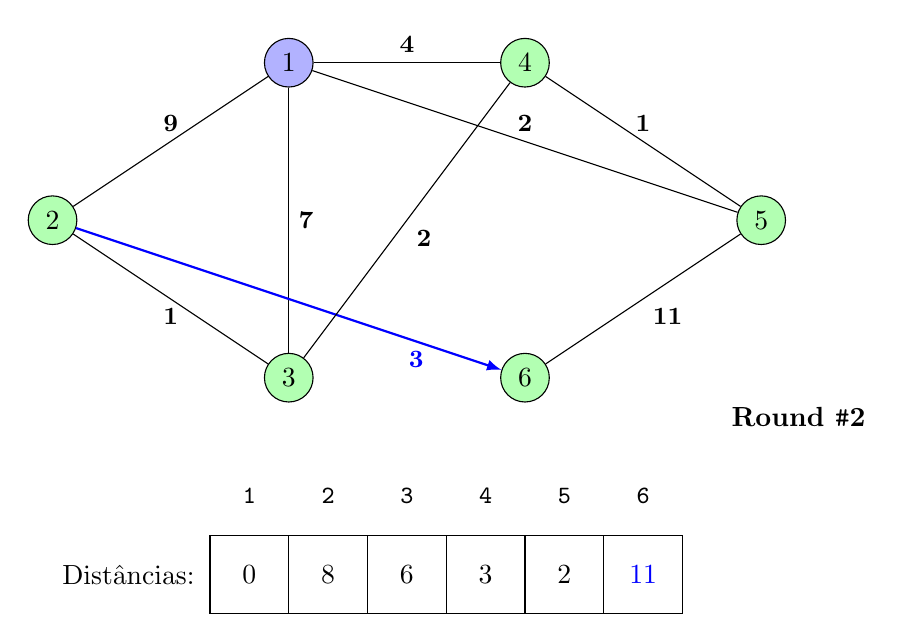
\begin{tikzpicture}
        \node[anchor=west] at (0, 0.5) { Distâncias: };
        \node[anchor=west] at (8.5, 2.5) { \bfseries Round \texttt{\#}2 };

        \node[circle, draw, fill=blue!30] (a) at (3, 7) {1};
        \node[circle, draw, fill=green!30] (b) at (0, 5) {2};
        \node[circle, draw, fill=green!30] (c) at (3, 3) {3};
        \node[circle, draw, fill=green!30] (d) at (6, 7) {4};
        \node[circle, draw, fill=green!30] (e) at (9, 5) {5};
        \node[circle, draw, fill=green!30] (f) at (6, 3) {6};

        \draw (2, 0) grid (8, 1);

        \node at (2.5, 0.5) { $0$ };
        \node at (3.5, 0.5) { \textcolor{black}{$8$} };
        \node at (4.5, 0.5) { \textcolor{black}{$6$} };
        \node at (5.5, 0.5) { \textcolor{black}{$3$} };
        \node at (6.5, 0.5) { \textcolor{black}{$2$} };
        \node at (7.5, 0.5) { \textcolor{blue}{$11$} };

        \node at (2.5, 1.5) { \small \texttt{1} };
        \node at (3.5, 1.5) { \small \texttt{2} };
        \node at (4.5, 1.5) { \small \texttt{3} };
        \node at (5.5, 1.5) { \small \texttt{4} };
        \node at (6.5, 1.5) { \small \texttt{5} };
        \node at (7.5, 1.5) { \small \texttt{6} };

        \draw (a) to node[midway,anchor=south] { \small \bfseries 9 } (b);
        \draw (a) to node[midway,anchor=west] { \small \bfseries 7 } (c);
        \draw (a) to node[midway,anchor=south] { \small \bfseries 4 } (d);
        \draw (a) to node[midway,anchor=south] { \small \bfseries 2 } (e);
        \draw (b) to node[midway,anchor=north] { \small \bfseries 1 } (c);
        \draw[-latex,thick,blue] (b) to node[pos=0.8,anchor=north] { \small \bfseries 3 } (f);
        \draw (c) to node[midway,anchor=north west] { \small \bfseries 2 } (d);
        \draw (d) to node[midway,anchor=south] { \small \bfseries 1 } (e);
        \draw (e) to node[midway,anchor=north west] { \small \bfseries 11 } (f);

    \end{tikzpicture}

\end{frame}

\begin{frame}[fragile]{Visualização do algoritmo de Bellman-Ford}

    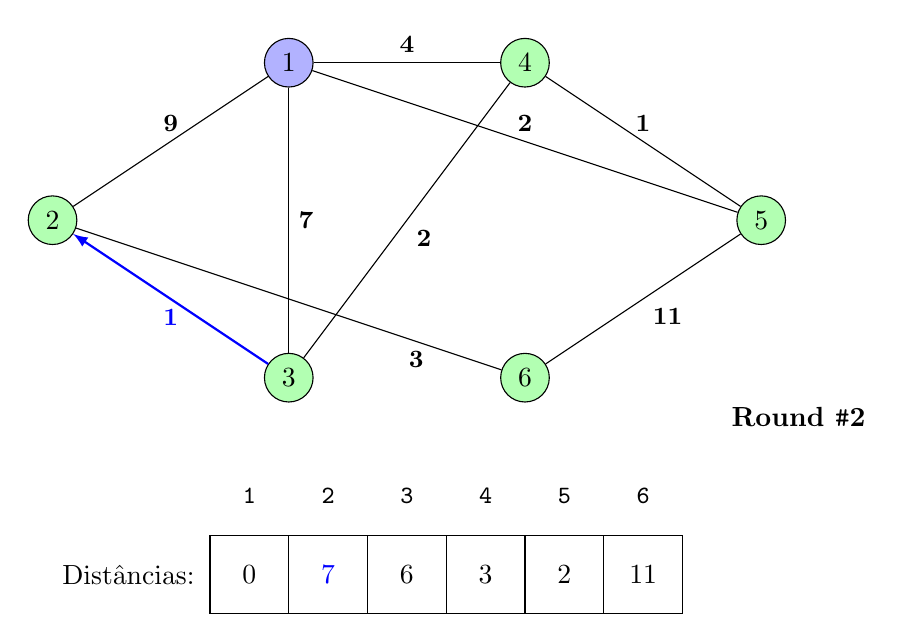
\begin{tikzpicture}
        \node[anchor=west] at (0, 0.5) { Distâncias: };
        \node[anchor=west] at (8.5, 2.5) { \bfseries Round \texttt{\#}2 };

        \node[circle, draw, fill=blue!30] (a) at (3, 7) {1};
        \node[circle, draw, fill=green!30] (b) at (0, 5) {2};
        \node[circle, draw, fill=green!30] (c) at (3, 3) {3};
        \node[circle, draw, fill=green!30] (d) at (6, 7) {4};
        \node[circle, draw, fill=green!30] (e) at (9, 5) {5};
        \node[circle, draw, fill=green!30] (f) at (6, 3) {6};

        \draw (2, 0) grid (8, 1);

        \node at (2.5, 0.5) { $0$ };
        \node at (3.5, 0.5) { \textcolor{blue}{$7$} };
        \node at (4.5, 0.5) { \textcolor{black}{$6$} };
        \node at (5.5, 0.5) { \textcolor{black}{$3$} };
        \node at (6.5, 0.5) { \textcolor{black}{$2$} };
        \node at (7.5, 0.5) { \textcolor{black}{$11$} };

        \node at (2.5, 1.5) { \small \texttt{1} };
        \node at (3.5, 1.5) { \small \texttt{2} };
        \node at (4.5, 1.5) { \small \texttt{3} };
        \node at (5.5, 1.5) { \small \texttt{4} };
        \node at (6.5, 1.5) { \small \texttt{5} };
        \node at (7.5, 1.5) { \small \texttt{6} };

        \draw (a) to node[midway,anchor=south] { \small \bfseries 9 } (b);
        \draw (a) to node[midway,anchor=west] { \small \bfseries 7 } (c);
        \draw (a) to node[midway,anchor=south] { \small \bfseries 4 } (d);
        \draw (a) to node[midway,anchor=south] { \small \bfseries 2 } (e);
        %\draw (b) to node[midway,anchor=north] { \small \bfseries 1 } (c);
        \draw[latex-,thick,blue](b) to node[midway,anchor=north] { \small \bfseries 1 } (c);
        \draw (b) to node[pos=0.8,anchor=north] { \small \bfseries 3 } (f);
        \draw (c) to node[midway,anchor=north west] { \small \bfseries 2 } (d);
        \draw (d) to node[midway,anchor=south] { \small \bfseries 1 } (e);
        \draw (e) to node[midway,anchor=north west] { \small \bfseries 11 } (f);

    \end{tikzpicture}

\end{frame}

\begin{frame}[fragile]{Visualização do algoritmo de Bellman-Ford}

    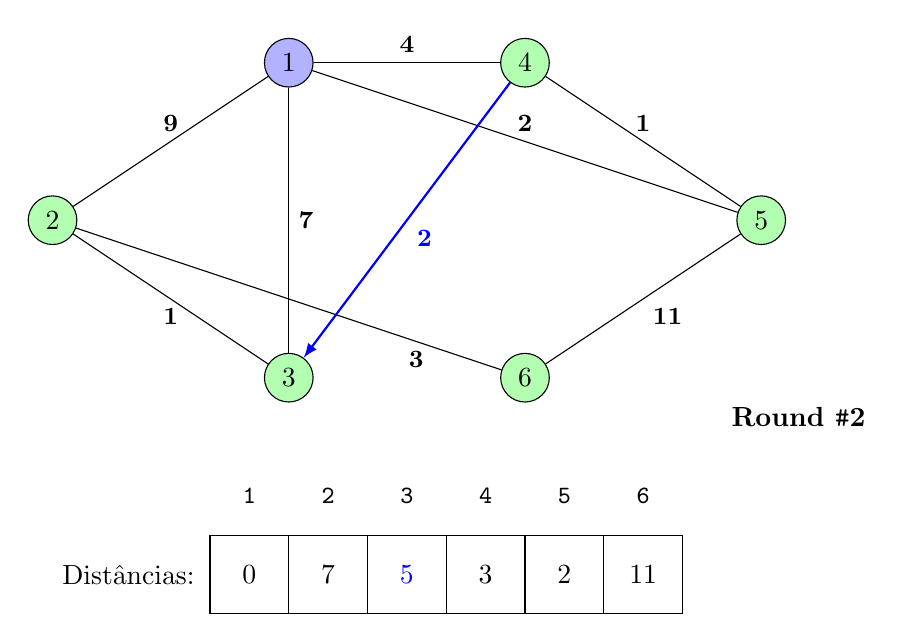
\begin{tikzpicture}
        \node[anchor=west] at (0, 0.5) { Distâncias: };
        \node[anchor=west] at (8.5, 2.5) { \bfseries Round \texttt{\#}2 };

        \node[circle, draw, fill=blue!30] (a) at (3, 7) {1};
        \node[circle, draw, fill=green!30] (b) at (0, 5) {2};
        \node[circle, draw, fill=green!30] (c) at (3, 3) {3};
        \node[circle, draw, fill=green!30] (d) at (6, 7) {4};
        \node[circle, draw, fill=green!30] (e) at (9, 5) {5};
        \node[circle, draw, fill=green!30] (f) at (6, 3) {6};

        \draw (2, 0) grid (8, 1);

        \node at (2.5, 0.5) { $0$ };
        \node at (3.5, 0.5) { \textcolor{black}{$7$} };
        \node at (4.5, 0.5) { \textcolor{blue}{$5$} };
        \node at (5.5, 0.5) { \textcolor{black}{$3$} };
        \node at (6.5, 0.5) { \textcolor{black}{$2$} };
        \node at (7.5, 0.5) { \textcolor{black}{$11$} };

        \node at (2.5, 1.5) { \small \texttt{1} };
        \node at (3.5, 1.5) { \small \texttt{2} };
        \node at (4.5, 1.5) { \small \texttt{3} };
        \node at (5.5, 1.5) { \small \texttt{4} };
        \node at (6.5, 1.5) { \small \texttt{5} };
        \node at (7.5, 1.5) { \small \texttt{6} };

        \draw (a) to node[midway,anchor=south] { \small \bfseries 9 } (b);
        \draw (a) to node[midway,anchor=west] { \small \bfseries 7 } (c);
        \draw (a) to node[midway,anchor=south] { \small \bfseries 4 } (d);
        \draw (a) to node[midway,anchor=south] { \small \bfseries 2 } (e);
        \draw (b) to node[midway,anchor=north] { \small \bfseries 1 } (c);
        \draw (b) to node[pos=0.8,anchor=north] { \small \bfseries 3 } (f);
        %\draw (c) to node[midway,anchor=north west] { \small \bfseries 2 } (d);
        \draw[latex-,thick,blue](c) to node[midway,anchor=north west] { \small \bfseries 2 } (d);
        \draw (d) to node[midway,anchor=south] { \small \bfseries 1 } (e);
        \draw (e) to node[midway,anchor=north west] { \small \bfseries 11 } (f);

    \end{tikzpicture}

\end{frame}

\begin{frame}[fragile]{Visualização do algoritmo de Bellman-Ford}

    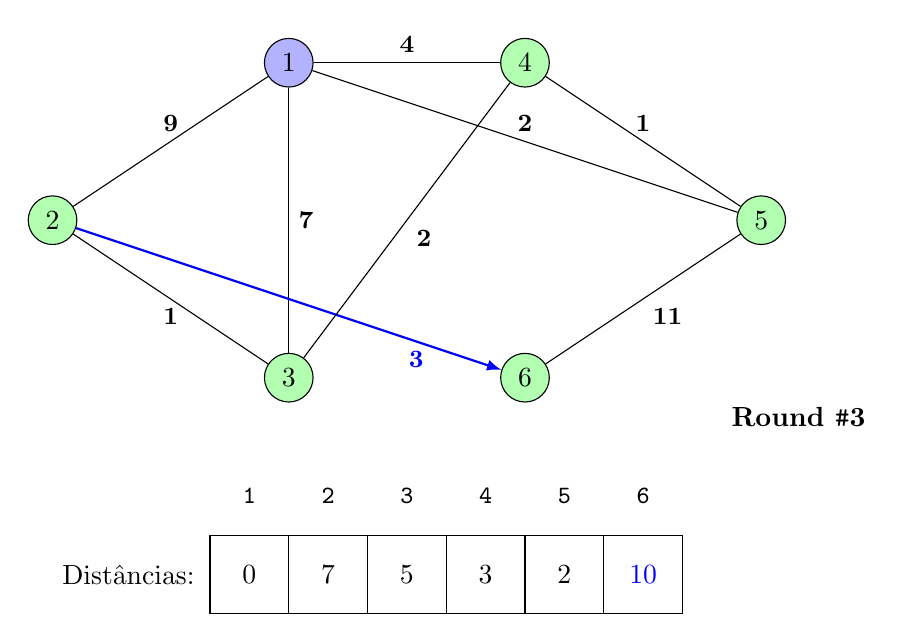
\begin{tikzpicture}
        \node[anchor=west] at (0, 0.5) { Distâncias: };
        \node[anchor=west] at (8.5, 2.5) { \bfseries Round \texttt{\#}3 };

        \node[circle, draw, fill=blue!30] (a) at (3, 7) {1};
        \node[circle, draw, fill=green!30] (b) at (0, 5) {2};
        \node[circle, draw, fill=green!30] (c) at (3, 3) {3};
        \node[circle, draw, fill=green!30] (d) at (6, 7) {4};
        \node[circle, draw, fill=green!30] (e) at (9, 5) {5};
        \node[circle, draw, fill=green!30] (f) at (6, 3) {6};

        \draw (2, 0) grid (8, 1);

        \node at (2.5, 0.5) { $0$ };
        \node at (3.5, 0.5) { \textcolor{black}{$7$} };
        \node at (4.5, 0.5) { \textcolor{black}{$5$} };
        \node at (5.5, 0.5) { \textcolor{black}{$3$} };
        \node at (6.5, 0.5) { \textcolor{black}{$2$} };
        \node at (7.5, 0.5) { \textcolor{blue}{$10$} };

        \node at (2.5, 1.5) { \small \texttt{1} };
        \node at (3.5, 1.5) { \small \texttt{2} };
        \node at (4.5, 1.5) { \small \texttt{3} };
        \node at (5.5, 1.5) { \small \texttt{4} };
        \node at (6.5, 1.5) { \small \texttt{5} };
        \node at (7.5, 1.5) { \small \texttt{6} };

        \draw (a) to node[midway,anchor=south] { \small \bfseries 9 } (b);
        \draw (a) to node[midway,anchor=west] { \small \bfseries 7 } (c);
        \draw (a) to node[midway,anchor=south] { \small \bfseries 4 } (d);
        \draw (a) to node[midway,anchor=south] { \small \bfseries 2 } (e);
        \draw (b) to node[midway,anchor=north] { \small \bfseries 1 } (c);
        %\draw (b) to node[pos=0.8,anchor=north] { \small \bfseries 3 } (f);
        \draw[-latex,thick,blue] (b) to node[pos=0.8,anchor=north] { \small \bfseries 3 } (f);
        \draw (c) to node[midway,anchor=north west] { \small \bfseries 2 } (d);
        \draw (d) to node[midway,anchor=south] { \small \bfseries 1 } (e);
        \draw (e) to node[midway,anchor=north west] { \small \bfseries 11 } (f);

    \end{tikzpicture}

\end{frame}

\begin{frame}[fragile]{Visualização do algoritmo de Bellman-Ford}

    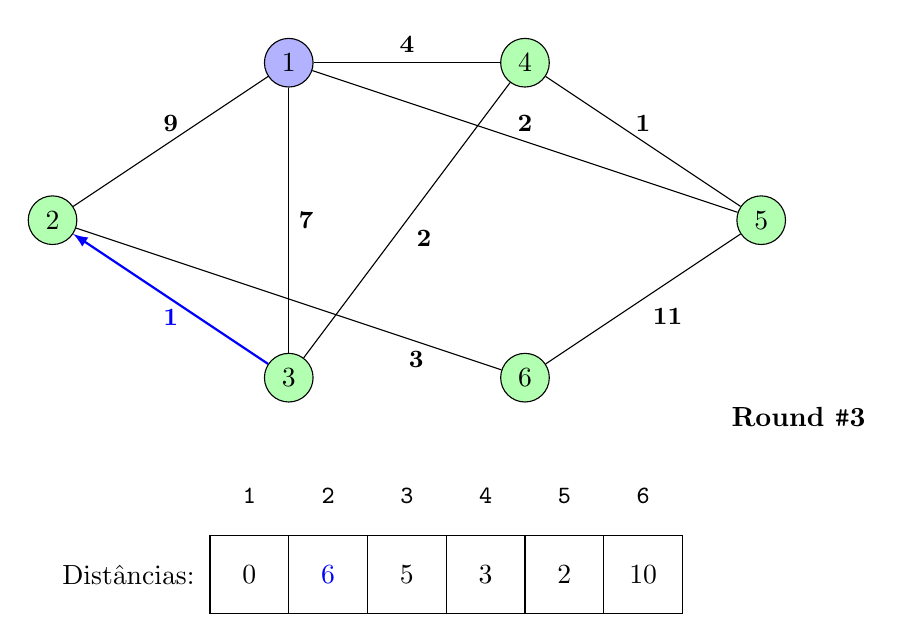
\begin{tikzpicture}
        \node[anchor=west] at (0, 0.5) { Distâncias: };
        \node[anchor=west] at (8.5, 2.5) { \bfseries Round \texttt{\#}3 };

        \node[circle, draw, fill=blue!30] (a) at (3, 7) {1};
        \node[circle, draw, fill=green!30] (b) at (0, 5) {2};
        \node[circle, draw, fill=green!30] (c) at (3, 3) {3};
        \node[circle, draw, fill=green!30] (d) at (6, 7) {4};
        \node[circle, draw, fill=green!30] (e) at (9, 5) {5};
        \node[circle, draw, fill=green!30] (f) at (6, 3) {6};

        \draw (2, 0) grid (8, 1);

        \node at (2.5, 0.5) { $0$ };
        \node at (3.5, 0.5) { \textcolor{blue}{$6$} };
        \node at (4.5, 0.5) { \textcolor{black}{$5$} };
        \node at (5.5, 0.5) { \textcolor{black}{$3$} };
        \node at (6.5, 0.5) { \textcolor{black}{$2$} };
        \node at (7.5, 0.5) { \textcolor{black}{$10$} };

        \node at (2.5, 1.5) { \small \texttt{1} };
        \node at (3.5, 1.5) { \small \texttt{2} };
        \node at (4.5, 1.5) { \small \texttt{3} };
        \node at (5.5, 1.5) { \small \texttt{4} };
        \node at (6.5, 1.5) { \small \texttt{5} };
        \node at (7.5, 1.5) { \small \texttt{6} };

        \draw (a) to node[midway,anchor=south] { \small \bfseries 9 } (b);
        \draw (a) to node[midway,anchor=west] { \small \bfseries 7 } (c);
        \draw (a) to node[midway,anchor=south] { \small \bfseries 4 } (d);
        \draw (a) to node[midway,anchor=south] { \small \bfseries 2 } (e);
        %\draw (b) to node[midway,anchor=north] { \small \bfseries 1 } (c);
        \draw[latex-,thick,blue] (b) to node[midway,anchor=north] { \small \bfseries 1 } (c);
        \draw (b) to node[pos=0.8,anchor=north] { \small \bfseries 3 } (f);
        \draw (c) to node[midway,anchor=north west] { \small \bfseries 2 } (d);
        \draw (d) to node[midway,anchor=south] { \small \bfseries 1 } (e);
        \draw (e) to node[midway,anchor=north west] { \small \bfseries 11 } (f);

    \end{tikzpicture}

\end{frame}

\begin{frame}[fragile]{Visualização do algoritmo de Bellman-Ford}

    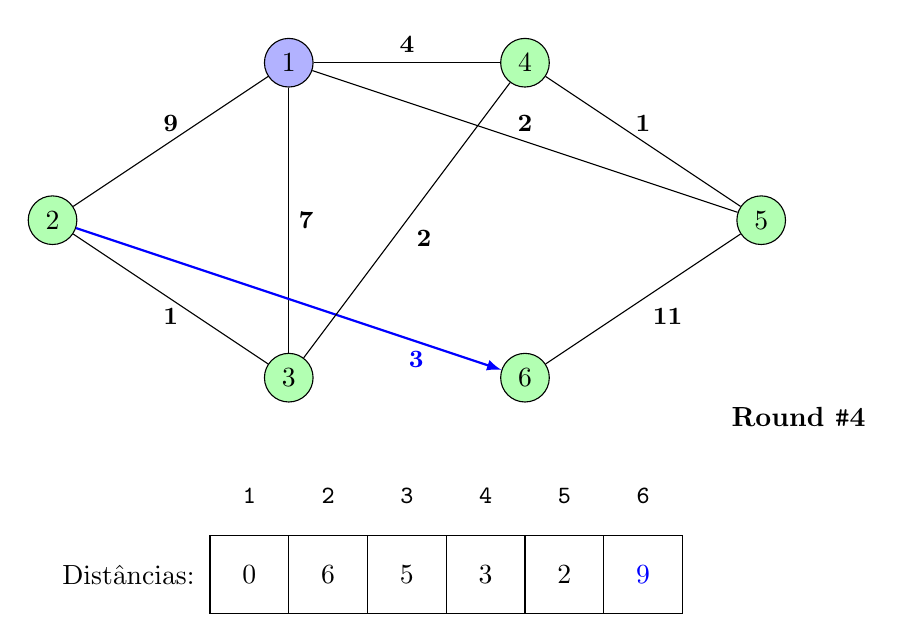
\begin{tikzpicture}
        \node[anchor=west] at (0, 0.5) { Distâncias: };
        \node[anchor=west] at (8.5, 2.5) { \bfseries Round \texttt{\#}4 };

        \node[circle, draw, fill=blue!30] (a) at (3, 7) {1};
        \node[circle, draw, fill=green!30] (b) at (0, 5) {2};
        \node[circle, draw, fill=green!30] (c) at (3, 3) {3};
        \node[circle, draw, fill=green!30] (d) at (6, 7) {4};
        \node[circle, draw, fill=green!30] (e) at (9, 5) {5};
        \node[circle, draw, fill=green!30] (f) at (6, 3) {6};

        \draw (2, 0) grid (8, 1);

        \node at (2.5, 0.5) { $0$ };
        \node at (3.5, 0.5) { \textcolor{black}{$6$} };
        \node at (4.5, 0.5) { \textcolor{black}{$5$} };
        \node at (5.5, 0.5) { \textcolor{black}{$3$} };
        \node at (6.5, 0.5) { \textcolor{black}{$2$} };
        \node at (7.5, 0.5) { \textcolor{blue}{$9$} };

        \node at (2.5, 1.5) { \small \texttt{1} };
        \node at (3.5, 1.5) { \small \texttt{2} };
        \node at (4.5, 1.5) { \small \texttt{3} };
        \node at (5.5, 1.5) { \small \texttt{4} };
        \node at (6.5, 1.5) { \small \texttt{5} };
        \node at (7.5, 1.5) { \small \texttt{6} };

        \draw (a) to node[midway,anchor=south] { \small \bfseries 9 } (b);
        \draw (a) to node[midway,anchor=west] { \small \bfseries 7 } (c);
        \draw (a) to node[midway,anchor=south] { \small \bfseries 4 } (d);
        \draw (a) to node[midway,anchor=south] { \small \bfseries 2 } (e);
        \draw (b) to node[midway,anchor=north] { \small \bfseries 1 } (c);
        %\draw (b) to node[pos=0.8,anchor=north] { \small \bfseries 3 } (f);
        \draw[-latex,thick,blue] (b) to node[pos=0.8,anchor=north] { \small \bfseries 3 } (f);
        \draw (c) to node[midway,anchor=north west] { \small \bfseries 2 } (d);
        \draw (d) to node[midway,anchor=south] { \small \bfseries 1 } (e);
        \draw (e) to node[midway,anchor=north west] { \small \bfseries 11 } (f);

    \end{tikzpicture}

\end{frame}

\begin{frame}[fragile]{Implementação de Bellman-Ford em C++}
    \inputsnippet{cpp}{1}{20}{bellman-ford.cpp}
\end{frame}

\begin{frame}[fragile]{Implementação de Bellman-Ford em C++}
    \inputsnippet{cpp}{21}{40}{bellman-ford.cpp}
\end{frame}


\begin{frame}[fragile]{Identificação do caminho mínimo}

    \begin{itemize}
        \item A implementação do algoritmo de Bellman-Ford apresentada computa a distância
            mínima entre qualquer vértice $u$ conectado ao vértice $s$, mas não determina
            qual seria este caminho

        \item Para determinar o caminho, é preciso manter o vetor \code{c++}{pred}, onde
            \code{c++}{pred[u]} é o nó que antecede $u$ no caminho mínimo que vai de $s$ a 
            $u$

        \item Inicialmente, todos os elementos deste vetor devem ser iguais a um valor sentinela,
            exceto o vértice $s$, que terá \code{c++}{pred[s] = s}

        \item Se a aresta $(u, v)$ atualizar a distância \code{c++}{dist[v]}, então o 
            predecessor deve ser atualizado também: \code{c++}{pred[v] = u}

        \item Deste modo, o caminho pode ser recuperado, passando por todos os predecessores até
            se atingir o nó um

        \item Se o predecessor de $u$ for o valor sentinela, não há caminho de $s$ a $u$ no
            grafo
    \end{itemize}

\end{frame}

\begin{frame}[fragile]{Implementação da identificação do caminho mínimo em C++}
    \inputsnippet{c++}{1}{17}{bellman-ford2.cpp}
\end{frame}

\begin{frame}[fragile]{Implementação da identificação do caminho mínimo em C++}
    \inputsnippet{c++}{18}{38}{bellman-ford2.cpp}
\end{frame}

\begin{frame}[fragile]{Implementação da identificação do caminho mínimo em C++}
    \inputsnippet{c++}{40}{60}{bellman-ford2.cpp}
\end{frame}

\begin{frame}[fragile]{Ciclos negativos}

    \begin{itemize}
        \item Um grafo $G$ tem um ciclo negativo quando a soma dos pesos das arestas de um
            ciclo resultam em um valor menor do que zero

        \item A presença de um ciclo negativo faz com que, a cada iteração, o algoritmo de
            Bellman-Ford atualize ao menos uma distância

        \item Desta forma, o próprio algoritmo pode ser usado para detectar tais ciclos

        \item Basta iterar o algoritmo mais uma vez após o seu término: caso o algoritmo faça
            alguma atualização nas distâncias, há um ciclo negativo no grafo

        \item Tal estratégia identificará tais ciclos no componente conectado do grafo, 
            independentemente do nó inicial escolhido
    \end{itemize}

\end{frame}

\begin{frame}[fragile]{Implementação da identificação de ciclos negativos}
    \inputsnippet{c++}{9}{25}{negative_cycle.cpp}
\end{frame}
